%%%%%%%%%%%%%%%%%%%%%%%%%%%%%%%%%%%%%%%%%%%%%%%%%%%%%%%%%%%%%%%%%%%%%%%%
%% Customizações do abnTeX2 (http://abnTeX2.googlecode.com)           %%
%% para a Universidade de Fortaleza						              %%
%%                                                                    %%
%% This work may be distributed and/or modified under the             %%
%% conditions of the LaTeX Project Public License, either version 1.3 %%
%% of this license or (at your option) any later version.             %%
%% The latest version of this license is in                           %%
%%   http://www.latex-project.org/lppl.txt                            %%
%% and version 1.3 or later is part of all distributions of LaTeX     %%
%% version 2005/12/01 or later.                                       %%
%%                                                                    %%
%% This work has the LPPL maintenance status `maintained'.            %%
%%                                                                    %%
%% The Current Maintainer of this work is Bruno Lopes                 %%
%%                                                                    %%
%% Project available on: https://github.com/bruno-unifor/unifortex2   %%
%%                                                                    %%
%% Further information about abnTeX2                                  %%
%% are available on http://abntex2.googlecode.com/                    %%
%%                                                                    %%
%%%%%%%%%%%%%%%%%%%%%%%%%%%%%%%%%%%%%%%%%%%%%%%%%%%%%%%%%%%%%%%%%%%%%%%%

%%%%%%%%%%%%%%%%%%%%%%%%%%%%%%%%%%%%%%%%%%%%%%%%%%%%%%%%%%%%%%%%%%%%%%%%
%% Customizações do abnTeX2 (http://abnTeX2.googlecode.com)           %%
%% para a Universidade de Fortaleza						              %%
%%                                                                    %%
%% This work may be distributed and/or modified under the             %%
%% conditions of the LaTeX Project Public License, either version 1.3 %%
%% of this license or (at your option) any later version.             %%
%% The latest version of this license is in                           %%
%%   http://www.latex-project.org/lppl.txt                            %%
%% and version 1.3 or later is part of all distributions of LaTeX     %%
%% version 2005/12/01 or later.                                       %%
%%                                                                    %%
%% This work has the LPPL maintenance status `maintained'.            %%
%%                                                                    %%
%% The Current Maintainer of this work is Bruno Lopes                 %%
%%                                                                    %%
%% Project available on: https://github.com/bruno-unifor/unifortex2   %%
%%                                                                    %%
%% Further information about abnTeX2                                  %%
%% are available on http://abntex2.googlecode.com/                    %%
%%                                                                    %%
%%%%%%%%%%%%%%%%%%%%%%%%%%%%%%%%%%%%%%%%%%%%%%%%%%%%%%%%%%%%%%%%%%%%%%%%

\documentclass[
    a4paper,          % Tamanho da folha A4
    12pt,             % Tamanho da fonte 12pt
    chapter=TITLE,    % Todos os capitulos devem ter caixa alta
    section=TITLE,    % Todas as secoes devem ter caixa alta
    oneside,          % Usada para impressao em apenas uma face do papel
    english,          % Hifenizacoes em ingles
    spanish,          % Hifenizacoes em espanhol
    brazilian         % Ultimo idioma eh o idioma padrao do documento
]{abntex2}

% Importações de pacotes
\usepackage[brazilian]{babel}
\usepackage[utf8]{inputenc}                         % Acentuação direta
\usepackage[T1]{fontenc}                            % Codificação da fonte em 8 bits
\usepackage{graphicx}                               % Inserir figuras
% Gráficos gerados a partir dos CSV em article/figuras/dados/, produzidos por
% `uv run python -m src.evaluation.export_figuras`. Nenhum número das figuras é
% transcrito à mão: reexecutar um braço e rodar o script regenera tudo.
\usepackage{pgfplots}
\pgfplotsset{compat=1.18}
\usepgfplotslibrary{statistics}
% Diagramas BPMN qualitativos, gerados por `src.evaluation.bpmn_tikz` a partir
% do BPMNDI do próprio pipeline — o leiaute mostrado é o que o sistema produz.
\usetikzlibrary{shapes.geometric, arrows.meta}
% Paleta validada para daltonismo (deuteranopia/tritanopia) — ΔE mínimo 11,6
% entre pares adjacentes. Toda figura usa também codificação secundária
% (traçado ou marcador), para o caso de impressão em tons de cinza.
\definecolor{corXML}{HTML}{1B6EC2}
\definecolor{corDSL}{HTML}{D95F02}
\definecolor{corSFT}{HTML}{1B9E77}
\definecolor{corTeto}{HTML}{6B6B6B}
\usepackage{amsfonts, amssymb, amsmath}             % Fonte e símbolos matemáticos
\usepackage{booktabs}                               % Comandos para tabelas
\usepackage{verbatim}                               % Texto é interpretado como escrito no documento
\usepackage{multirow, array}                        % Múltiplas linhas e colunas em tabelas
\usepackage{indentfirst}                            % Endenta o primeiro parágrafo de cada seção.
\usepackage{listings}                               % Utilizar codigo fonte no documento
\usepackage{xcolor}
\usepackage{microtype}                              % Para melhorias de justificação?
\usepackage[portuguese,ruled,lined]{algorithm2e}    % Escrever algoritmos
\usepackage{algorithmic}                            % Criar Algoritmos
%\usepackage{float}                                  % Utilizado para criação de floats
\usepackage{amsgen}
\usepackage{lipsum}                                 % Usar a simulação de texto Lorem Ipsum
%\usepackage{titlesec}                               % Permite alterar os títulos do documento
\usepackage{tocloft}                                % Permite alterar a formatação do Sumário
\usepackage{etoolbox}                               % Usado para alterar a fonte da Section no Sumário
\usepackage[nogroupskip,nonumberlist,acronym]{glossaries}                % Permite fazer o glossario
\usepackage{caption}                                % Altera o comportamento da tag caption
\usepackage[alf, abnt-emphasize=bf, bibjustif, recuo=0cm, abnt-etal-cite=3, abnt-etal-list=0,abnt-etal-text=it]{abntex2cite}  % Citações padrão ABNT
%\usepackage[bottom]{footmisc}                      % Mantém as notas de rodapé sempre na mesma posição
%\usepackage{times}                                 % Usa a fonte Times
\usepackage{mathptmx}                               % Usa a fonte Times New Roman
%\usepackage{lmodern}                               % Usa a fonte Latin Modern
%\usepackage{subfig}                                % Posicionamento de figuras
%\usepackage{scalefnt}                              % Permite redimensionar tamanho da fonte
%\usepackage{color, colortbl}                       % Comandos de cores
%\usepackage{lscape}                                % Permite páginas em modo "paisagem"
%\usepackage{ae, aecompl}                           % Fontes de alta qualidade
%\usepackage{picinpar}                              % Dispor imagens em parágrafos
%\usepackage{latexsym}                              % Símbolos matemáticos
%\usepackage{upgreek}                               % Fonte letras gregas
\usepackage{appendix}                               % Gerar o apendice no final do documento
\usepackage{paracol}                                % Criar paragrafos sem identacao
\usepackage{lib/unifortex2}		                    % Biblioteca com as normas da Unifor para trabalhos academicos
\usepackage{pdfpages}                               % Incluir pdf no documento
\usepackage{amsmath}                                % Usar equacoes matematicas

% Organiza e gera a lista de abreviaturas, simbolos e glossario
% (o arquivo de siglas já é carregado por lib/unifortex2.sty)
\makeglossaries

% Gera o Indice do documento
\makeindex


%%%%%%%%%%%%%%%%%%%%%%%%%%%%%%%%%%%%%%%%%%%%%%%%%%%%%
%%          Configuracoes do uniforTeX2            %%
%%%%%%%%%%%%%%%%%%%%%%%%%%%%%%%%%%%%%%%%%%%%%%%%%%%%%

% Opcoes disponiveis

%% Trabalho final de GRADUAÇÃO no qual a folha de aprovação será um arquivo PDF
%\trabalhoacademico{tccgraduacaoPDF}

%% Trabalho final de GRADUAÇÃO no qual a folha de aprovação será gerada pelo modelo UniforTEX
\trabalhoacademico{tccgraduacao}

%% Trabalho final de ESPECIALIZAÇÃO no qual a folha de aprovação será gerada pelo modelo UniforTEX
%\trabalhoacademico{tccespecializacao}

%% Trabalho final de MESTRADO no qual a folha de aprovação será gerada pelo modelo UniforTEX
%\trabalhoacademico{dissertacao}

%% Trabalho final de DOUTORADO no qual a folha de aprovação será gerada pelo modelo UniforTEX
%\trabalhoacademico{tese}

% Define se o trabalho eh uma qualificacao
% Coloque 'nao' para versao final do trabalho

%\ehqualificacao{nao}

% Remove as bordas vermelhas e verdes do PDF gerado
% Coloque 'sim' pare remover

\removerbordasdohyperlink{sim}

% Adiciona a cor Azul a todos os hyperlinks

\cordohyperlink{nao}

%%%%%%%%%%%%%%%%%%%%%%%%%%%%%%%%%%%%%%%%%%%%%%%%%%%%%
%%          Informação sobre a IES                 %%
%%%%%%%%%%%%%%%%%%%%%%%%%%%%%%%%%%%%%%%%%%%%%%%%%%%%%

\ies{Universidade de Fortaleza}
\iessigla{UNIFOR}
\centro{Centro de Ciências Tecnológicas}

%%%%%%%%%%%%%%%%%%%%%%%%%%%%%%%%%%%%%%%%%%%%%%%%%%%%%
%%        Informação para TCC de Graduacao         %%
%%%%%%%%%%%%%%%%%%%%%%%%%%%%%%%%%%%%%%%%%%%%%%%%%%%%%

\graduacaoem{Ciência da Computação}
\habilitacao{bacharel} % Pode colocar tambem 'licenciada'

%%%%%%%%%%%%%%%%%%%%%%%%%%%%%%%%%%%%%%%%%%%%%%%%%%%%%
%%     Informação para TCC de Especializacao       %%
%%%%%%%%%%%%%%%%%%%%%%%%%%%%%%%%%%%%%%%%%%%%%%%%%%%%%

\especializacaoem{Alfabetização de Crianças}

%%%%%%%%%%%%%%%%%%%%%%%%%%%%%%%%%%%%%%%%%%%%%%%%%%%%%
%%         Informação para Dissertacao             %%
%%%%%%%%%%%%%%%%%%%%%%%%%%%%%%%%%%%%%%%%%%%%%%%%%%%%%

\programamestrado{Programa de Pós-Graduação em Informática Aplicada}
\nomedomestrado{Mestrado Acadêmico em Ciência da Computação}
\mestreem{Ciência da Computação}
\areadeconcentracaomestrado{Ciência da Computação}

%%%%%%%%%%%%%%%%%%%%%%%%%%%%%%%%%%%%%%%%%%%%%%%%%%%%%
%%               Informação para Tese              %%
%%%%%%%%%%%%%%%%%%%%%%%%%%%%%%%%%%%%%%%%%%%%%%%%%%%%%

\programadoutorado{Programa de Pós-Graduação em Informática Aplicada}
\nomedodoutorado{Doutorado em Saúde Coletiva}
\doutorem{Saúde Coletiva}
\areadeconcentracaodoutorado{Saúde Coletiva}

%%%%%%%%%%%%%%%%%%%%%%%%%%%%%%%%%%%%%%%%%%%%%%
%%  Informação relacionadas ao trabalho     %%
%%%%%%%%%%%%%%%%%%%%%%%%%%%%%%%%%%%%%%%%%%%%%%

\autor{Rafael Marins Florenzano}
% TODO: título provisório — revisar com o orientador antes da entrega
\titulo{Compressão Semântica na Geração de Modelos BPMN 2.0 \\ por Modelos de Linguagem: DSL e Transpilação Determinística}
\data{2026}
\local{Fortaleza -- Ceará}

% TODO: preencher com a data real da defesa
% Exemplo: \dataaprovacao{01 de Janeiro de 2017}
\dataaprovacao{}

%%%%%%%%%%%%%%%%%%%%%%%%%%%%%%%%%%%%%%%%%%%%%
%%     Informação sobre o Orientador       %%
%%%%%%%%%%%%%%%%%%%%%%%%%%%%%%%%%%%%%%%%%%%%%

% TODO: confirmar titulação do orientador (Me./Dr.)
\orientador{Prof. Caio Marques}
\orientadories{Universidade de Fortaleza - UNIFOR}
\orientadorcentro{Centro de Ciências Tecnológicas - CCT}
\orientadorfeminino{nao} % Coloque 'sim' se for do sexo feminino

%%%%%%%%%%%%%%%%%%%%%%%%%%%%%%%%%%%%%%%%%%%%%
%%      Informação sobre o Co-orientador   %%
%%%%%%%%%%%%%%%%%%%%%%%%%%%%%%%%%%%%%%%%%%%%%

% Deixe o nome do coorientador em branco para remover do documento

\coorientador{}
\coorientadories{Universidade Co-orientador - SIGLA}
\coorientadorcentro{Centro do Co-orientador - SIGLA}
\coorientadorfeminino{nao} % Coloque 'sim' se for do sexo feminino

%%%%%%%%%%%%%%%%%%%%%%%%%%%%%%%%%%%%%%%%%%%%%
%%      Informação sobre a banca           %%
%%%%%%%%%%%%%%%%%%%%%%%%%%%%%%%%%%%%%%%%%%%%%

% Atenção! Deixe o nome do membro da banca para remover da folha de aprovacao

% Exemplo de uso:
% \membrodabancadois{Prof. Dr. Fulano de Tal}
% \membrodabancadoisies{Universidade Estadual do Ceará - UECE}

\membrodabancadois{Membro da Banca Dois}
\membrodabancadoiscentro{Centro de Ciências e Tecnologia - CCT}
\membrodabancadoisies{Universidade do Membro da Banca Dois - SIGLA}

\membrodabancatres{Membro da Banca Três}
\membrodabancatrescentro{Centro de Ciências e Tecnologia - CCT}
\membrodabancatresies{Universidade do Membro da Banca Três - SIGLA}

\membrodabancaquatro{Membro da Banca Quatro}
\membrodabancaquatrocentro{Centro de Ciências e Tecnologia - CCT}
\membrodabancaquatroies{Universidade do Membro da Banca Quatro - SIGLA}

\membrodabancacinco{Membro da Banca Cinco}
\membrodabancacincocentro{Centro de Ciências e Tecnologia - CCT}
\membrodabancacincoies{Universidade do Membro da Banca Cinco - SIGLA}

\membrodabancaseis{Membro da Banca Seis}
\membrodabancaseiscentro{Centro de Ciências e Tecnologia - CCT}
\membrodabancaseisies{Universidade do Membro da Banca Seis - SIGLA}

\begin{document}

	% Elementos pré-textuais
	\imprimircapa
	\imprimirfolhaderosto{}
	\imprimirfichacatalografica{elementos-pre-textuais/ficha-catalografica}

	%%%%%%%%%%%%%%%%%%%%%%%%%%%%%%%%%%%%%%%%%%%%%%%%%%%%%%%%%%%%%%%%%%%%%%%%%%%%%%%%%%%%%%%%%%%%%%%%%%
	%%																                               	%%
	%%		Após a defesa do TCC, a banca examinadora irá preencher a folha de aprovação,			%%
	%%		que deverá ser assinada por todos os membros da banca avaliadora e, posteriormente,		%%
	%%		deverá ser anexada na versão final do TCC pelo ALUNO.									%%
	%%																								%%
	%%		Quando tiver em mãos a folha de aprovação:												%%
	%%			1 - Escanei-a e gere um arquivo PDF													%%
	%%			2 - Renomeie o arquivo PDF para "folha-aprovacao.pdf"								%%
	%%			3 - Mova o arquivo para o diretório "elementos-pre-textuais" do modelo				%%
	%%			5 - Descomente a linha 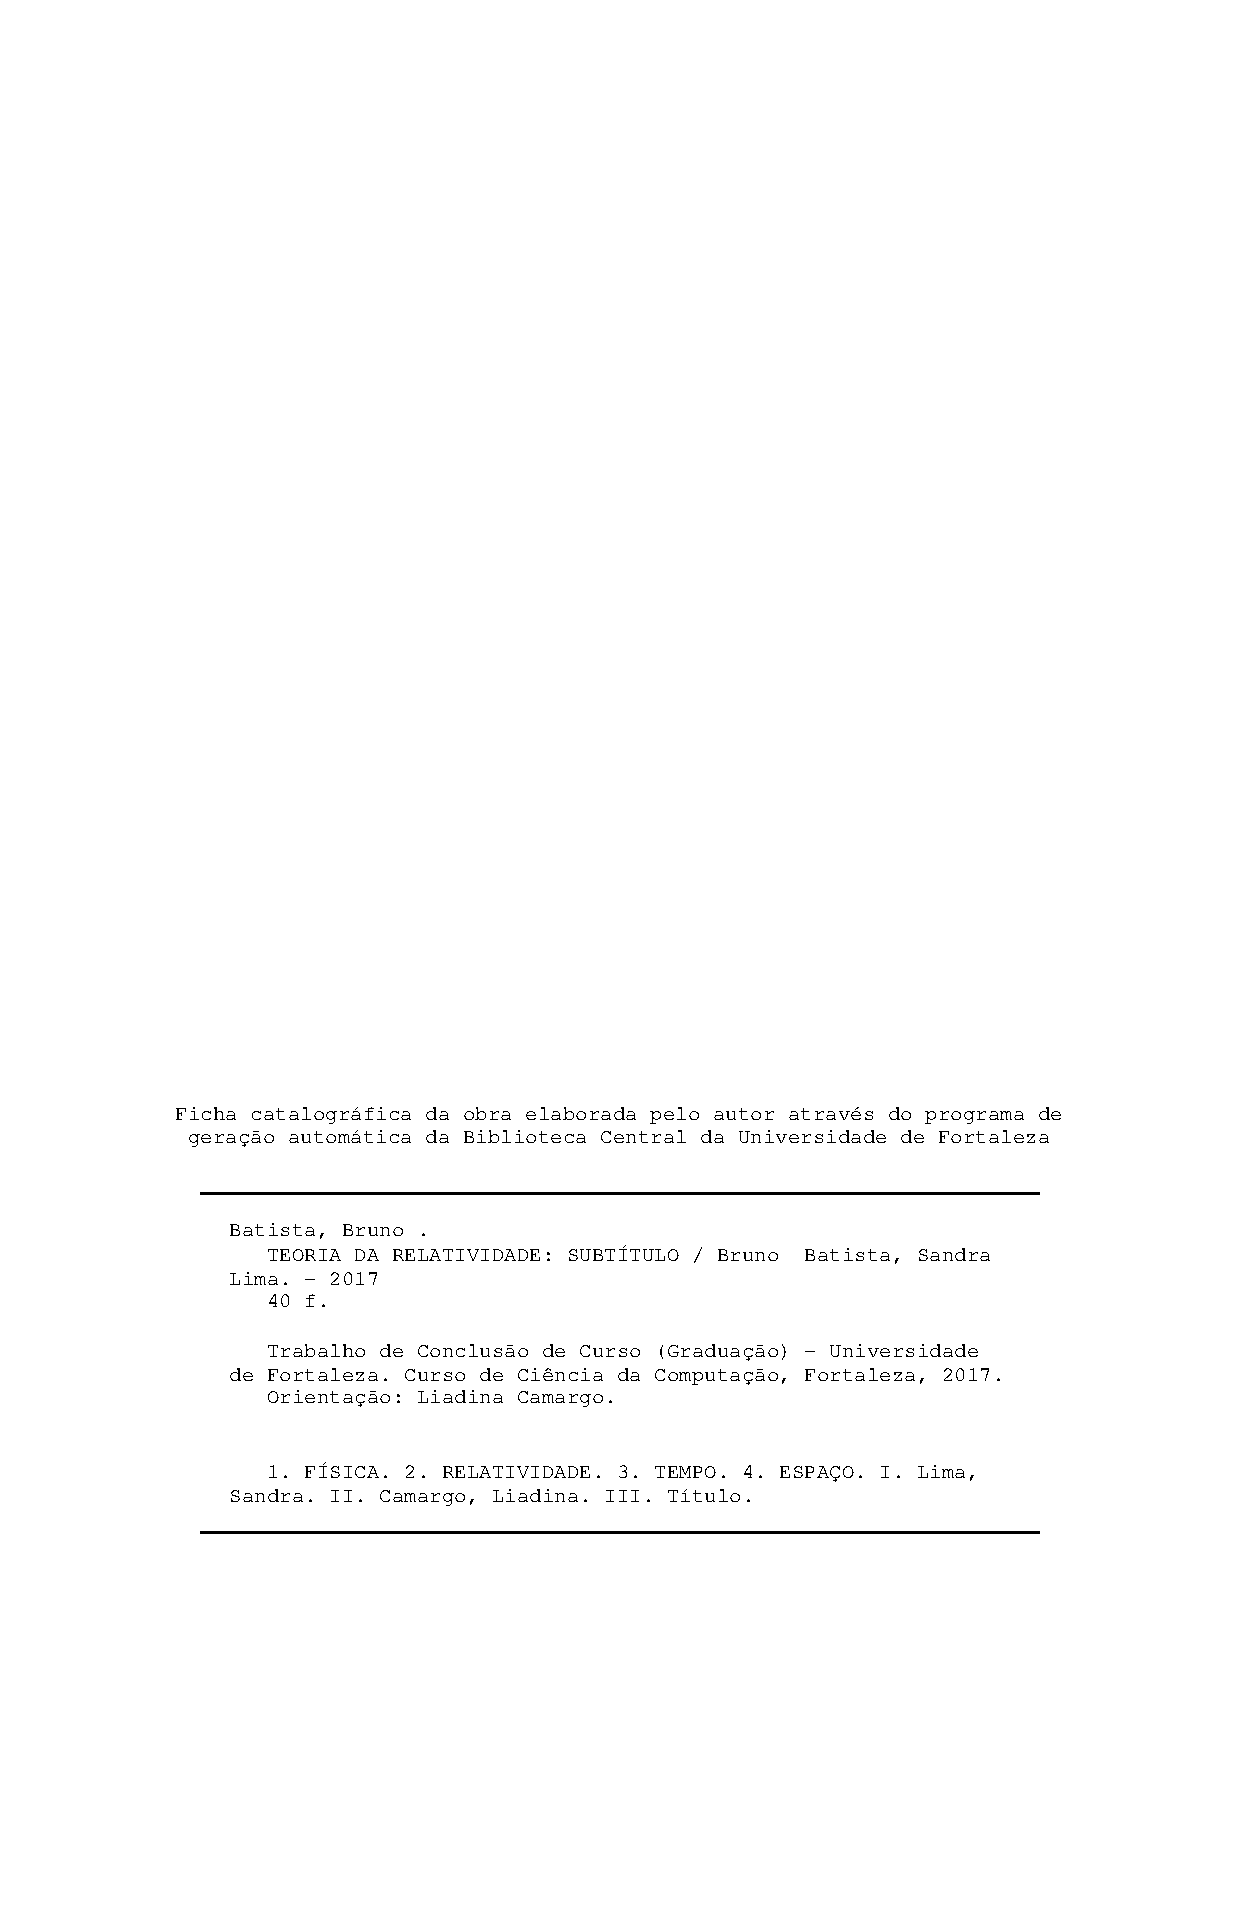
\includepdf{elementos-pre-textuais/folha-aprovacao.pdf} 		%%
	%%					removendo o simbolo de %													%%
	%%			6 - Adicione o simbolo % na linha 	\imprimirfolhadeaprovacao						%%
	%%			7 - Recompile o projeto																%%
	%%																								%%	%%%%%%%%%%%%%%%%%%%%%%%%%%%%%%%%%%%%%%%%%%%%%%%%%%%%%%%%%%%%%%%%%%%%%%%%%%%%%%%%%%%%%%%%%%%%%%%%%%
	
	%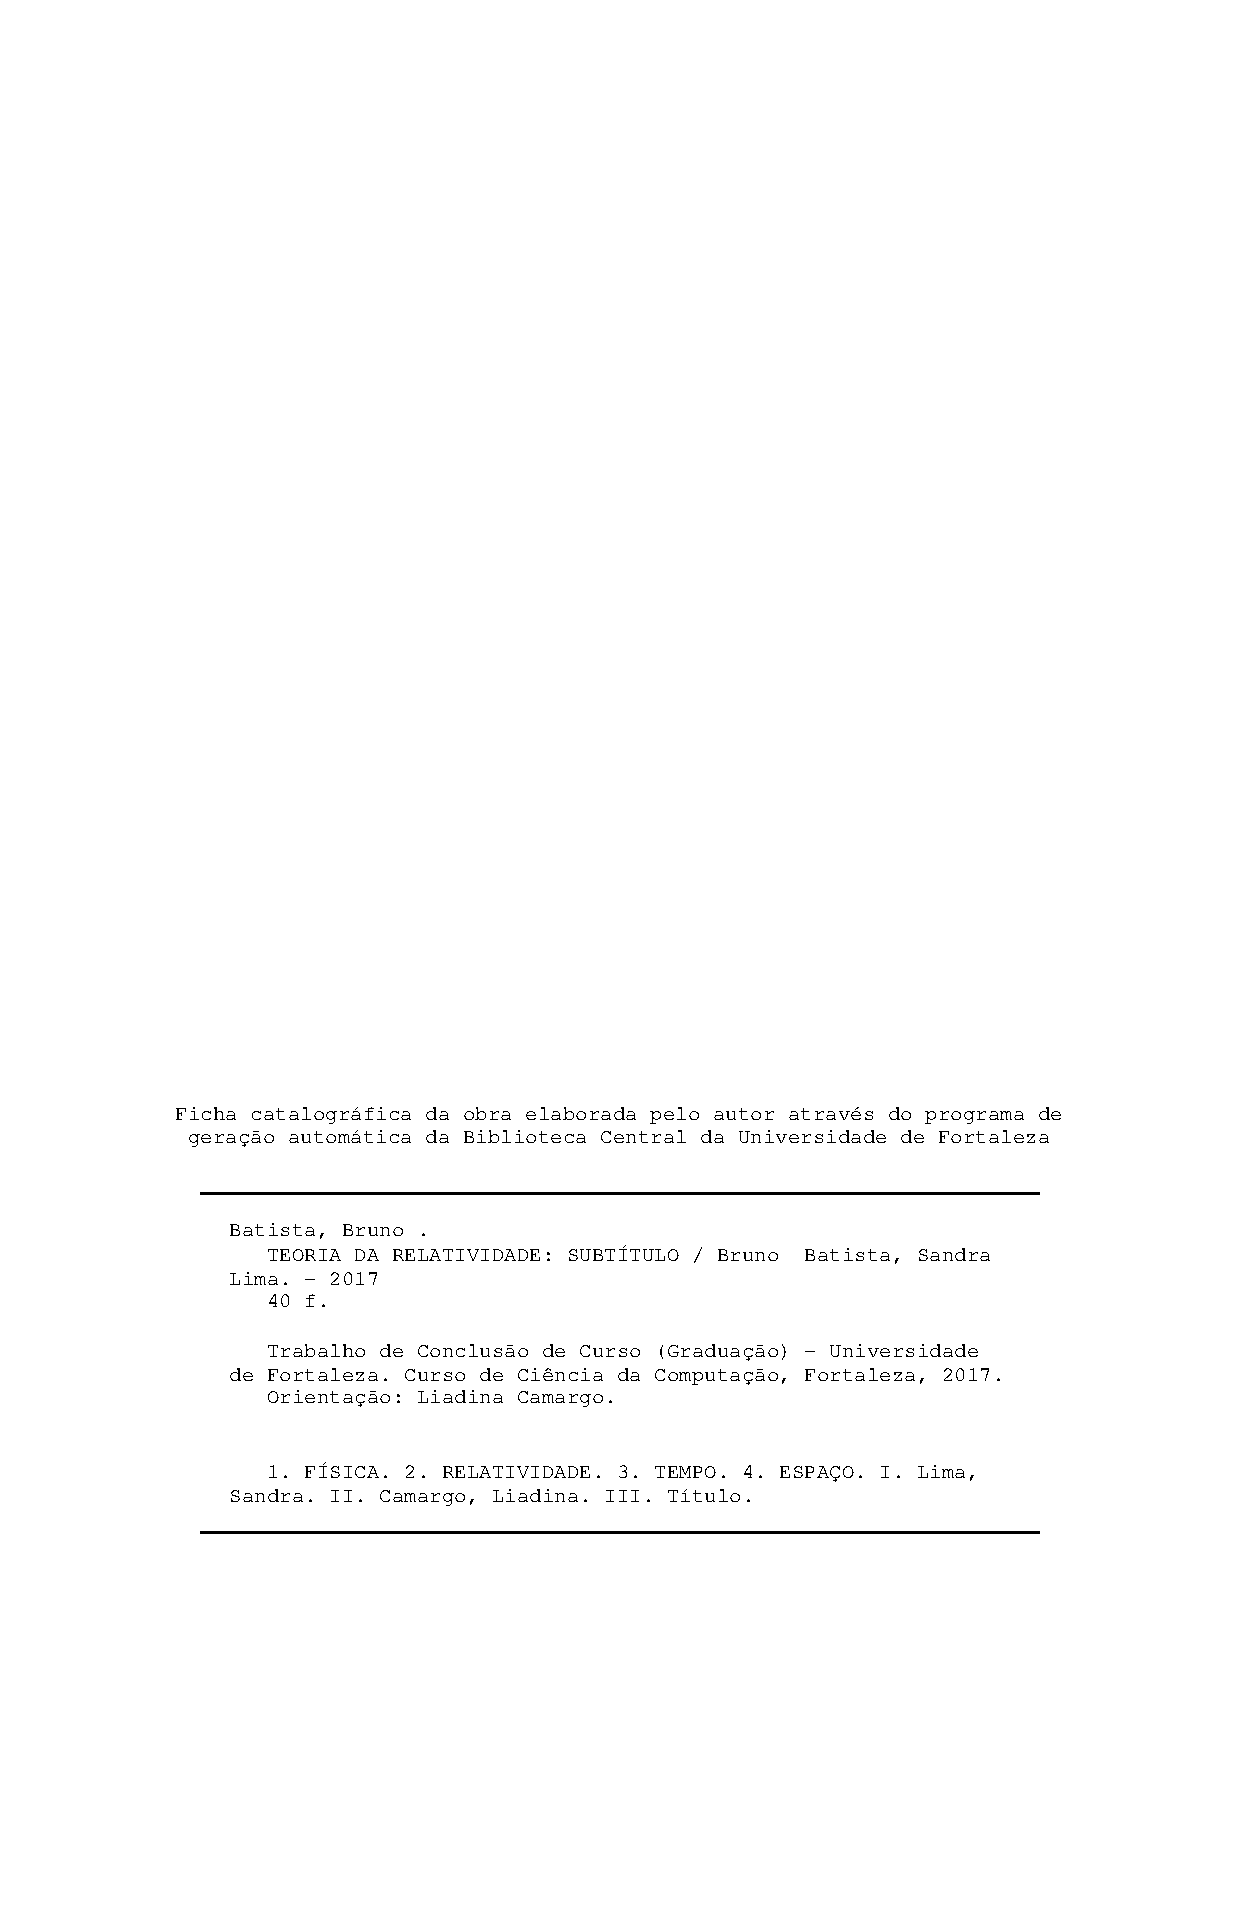
\includepdf{elementos-pre-textuais/folha-aprovacao.pdf}
	\imprimirfolhadeaprovacao
	
	% Dedicatória, agradecimentos, epígrafe e errata são opcionais na NBR 14724 e
	% foram removidos: o template os trazia preenchidos com o texto de exemplo de
	% outro TCC. Para reativar, restaurar a chamada e o arquivo correspondente em
	% elementos-pre-textuais/ (histórico no git).
	\imprimirresumo{elementos-pre-textuais/resumo}
	\imprimirabstract{elementos-pre-textuais/abstract}
	\imprimirlistadeilustracoes
	\imprimirlistadetabelas
	% Listas de quadros e de algoritmos suprimidas: o trabalho não usa nenhum dos
	% dois, e o template imprimia os dois títulos com a página em branco.
	\imprimirlistadecodigosfonte
	% O texto emprega as siglas em forma literal, sem marcação \gls, de modo que
	% nenhuma seria registrada como "usada" e a lista sairia vazia. \glsaddall
	% inclui todas as declaradas — e a lista declara apenas siglas que ocorrem
	% no texto, conferidas por contagem.
	\glsaddall
	\imprimirlistadeabreviaturasesiglas
	\imprimirlistadesimbolos{elementos-pre-textuais/lista-de-simbolos}
	\imprimirsumario

	%Elementos textuais
	\textual
	\chapter{Introdução}
\label{cap:introducao}

Organizações dependem de processos documentados para operar de forma previsível, treinar pessoas e cumprir exigências regulatórias. A notação BPMN 2.0, padronizada pela \citeonline{omg2011bpmn}, tornou-se a linguagem de referência para essa documentação, com uso consolidado tanto na indústria quanto na literatura de gestão de processos \cite{weske2019business, dumas2018fundamentals}. Na prática, porém, a maior parte do conhecimento sobre processos permanece registrada em linguagem natural: manuais internos, descrições de procedimentos e documentos de política. A conversão desse material em modelos formais continua sendo uma tarefa manual, lenta e dependente de especialistas \cite{friedrich2011process, vanderaa2018challenges}.

O avanço dos modelos de linguagem de grande porte \cite{vaswani2017attention, brown2020language} tornou plausível automatizar essa conversão. A dificuldade está na forma de saída. A serialização XML da BPMN foi concebida para intercâmbio entre ferramentas, não para ser escrita diretamente por pessoas ou por modelos. Ao solicitar que um modelo produza XML BPMN completo, transfere-se a ele uma responsabilidade pouco adequada ao seu funcionamento: reproduzir com precisão um grande volume de marcação técnica, ainda que boa parte dessa marcação possa ser derivada de maneira determinística. O custo aparece em duas frentes. A primeira é econômica e não depende de verificação: cada \textit{token} de marcação repetitiva consome contexto, tempo e dinheiro, e a quantidade emitida é diretamente mensurável. A segunda é de confiabilidade, e tem natureza distinta --- é uma \textbf{expectativa a ser testada}, não um dado. O risco existe em princípio, pois uma única inconsistência estrutural invalida o documento inteiro; se ele de fato se materializa, e em que medida, é questão empírica. Adianta-se que a resposta obtida neste trabalho contraria a expectativa inicial, conforme discutido adiante.

A redução do número de \textit{tokens} em sistemas baseados em modelos de linguagem tem sido atacada principalmente do lado da entrada. Na pesquisa, o LLMLingua \cite{jiang2023llmlingua} comprime o contexto antes que ele alcance o modelo, com ganhos expressivos e pouca perda de desempenho. Na indústria, ferramentas como o Headroom \cite{headroom2026} aplicam a mesma ideia a saídas de ferramentas, registros e trechos recuperados, relatando reduções entre 60\% e 95\% em conteúdo estruturado. Essas abordagens confirmam que a economia de \textit{tokens} é uma preocupação concreta e que boa parte dela vem da remoção de repetição estrutural. Nenhuma delas, entretanto, atua sobre o lado da geração: fazer com que o próprio modelo emita nativamente uma representação compacta, cuja expansão determinística produza um artefato válido segundo um esquema formal.

Duas linhas de trabalho se aproximam desse objetivo por caminhos distintos. A decodificação restrita, discutida por \citeonline{poesia2022synchromesh}, garante conformidade sintática durante a geração, mas não reduz o volume que o modelo precisa emitir. Já o ProMoAI, de \citeonline{kourani2024promoai}, gera modelos de processo por meio de uma representação intermediária expandida deterministicamente em BPMN, demonstrando que a estratégia é viável. O trabalho de \citeonline{kourani2024promoai} apoia-se, contudo, em um modelo de fronteira operado por \textit{prompt} e não trata a representação intermediária como um problema de compressão com taxa medida. É exatamente nesse espaço que esta monografia se posiciona.

A escolha do modelo também é parte do problema. \citeonline{belcak2025small} argumentam que modelos pequenos e especializados, e não modelos de fronteira genéricos, tendem a ser a base adequada para tarefas agênticas repetitivas, por razões de custo, latência e previsibilidade. Uma representação intermediária suficientemente compacta e regular torna essa especialização viável: reduz o que o modelo precisa aprender a emitir e permite que um modelo de sete bilhões de parâmetros, como o Qwen2.5-Coder \cite{hui2024qwen25coder}, seja ajustado para a tarefa.

Este trabalho propõe, portanto, um protocolo de compressão semântica para geração de BPMN. Um modelo de linguagem produz uma descrição concisa do processo em uma linguagem de domínio específico projetada para esse fim, e um transpilador baseado em gramática EBNF expande essa descrição em XML BPMN 2.0 validado contra o esquema oficial. A separação de responsabilidades traz um efeito colateral útil para a depuração: quando ocorre uma falha, ela fica localizada na geração da DSL, no transpilador ou na validação, em vez de diluída em um documento XML extenso. Medido sobre 1.021 processos com o tokenizador do Qwen2.5-Coder, o artefato proposto é \textbf{seis vezes} mais compacto que o XML lógico correspondente, o que equivale a uma redução de 83,4\% no número de \textit{tokens} que o modelo precisa emitir; sobre as saídas efetivamente geradas pelos braços experimentais, a razão sobe para cerca de sete.

Os resultados obtidos são antecipados aqui, por serem em parte contrários à expectativa que motivou o trabalho. A economia confirma-se sem ressalva. A confiabilidade, porém, depende de \textbf{como} a representação intermediária chega ao modelo. Descrita por \textit{prompt}, ela piora o desempenho: modelos de fronteira instruídos pela gramática produziram saída válida em 64,8\% e 56,6\% das gerações, contra 98,1\% e 94,3\% da geração direta de XML pelos mesmos modelos. Internalizada nos pesos por ajuste fino, ela melhora substancialmente: um modelo de sete bilhões de parâmetros atingiu 86,8\% de validade, vinte e dois pontos percentuais acima do modelo de fronteira instruído pela mesma gramática, embora ainda abaixo da geração direta. A explicação é que a serialização XML da BPMN, embora verbosa, é amplamente representada no pré-treinamento dos modelos, ao passo que a linguagem aqui proposta lhes é inteiramente nova --- verbosidade não constitui dificuldade para quem já viu o formato, novidade sim. Segue-se que o ajuste fino não é etapa acessória da abordagem, e sim condição de sua viabilidade.

Registra-se ainda um achado de ordem metodológica, obtido durante a avaliação e independente da linguagem proposta: mediu-se a concordância entre modelos de referência produzidos por especialistas distintos para o mesmo processo, e ela é baixa. Métricas estruturais que identificam nós por rótulo saturam, portanto, muito abaixo do máximo teórico, e todos os métodos avaliados operam nessa vizinhança. A consequência para a área é que valores absolutos dessas métricas não devem ser lidos como percentual de acerto.

\section{Motivação}
\label{sec:motivacao}

A modelagem de processos permanece cara justamente onde é mais necessária. Organizações que já documentam seus procedimentos em texto raramente dispõem de tempo especializado para convertê-los em modelos formais, e o resultado é uma base documental que não pode ser analisada, simulada ou automatizada. Reduzir o custo dessa conversão amplia o acesso à modelagem formal para além das organizações que podem manter analistas dedicados.

Há ainda uma motivação técnica, e ela independe do desfecho particular observado na BPMN. O padrão de separar a geração de uma representação compacta da expansão determinística em um artefato validável é aplicável a qualquer domínio em que a saída precise obedecer a um esquema formal e a serialização oficial seja verbosa. O que este trabalho tem a oferecer a esses domínios não é apenas a confirmação de um ganho, mas a identificação da \textbf{condição} sob a qual ele se realiza --- questão que só uma avaliação com protocolo previamente fixado poderia responder em qualquer direção. A BPMN oferece um caso de teste favorável para essa investigação porque possui esquema oficial, conjuntos de dados públicos com modelos de referência e métricas estruturais bem definidas, o que permite verificação objetiva em vez de avaliação subjetiva.

Por fim, a economia de \textit{tokens} deixou de ser detalhe de implementação. Em fluxos que geram modelos em escala, o custo de emitir marcação redundante é recorrente, e a alternativa de depender continuamente de modelos de fronteira concentra esse custo em um fornecedor externo. Um modelo pequeno ajustado para emitir uma representação comprimida é, nesse cenário, uma resposta de engenharia e não apenas um exercício acadêmico.

\section{Objetivos}
\label{sec:objetivos}

\subsection{Objetivo Geral}
\label{sec:objetivo-geral}

Investigar se a geração de uma representação intermediária comprimida, seguida de expansão determinística, produz modelos BPMN 2.0 válidos de forma mais confiável e mais econômica em \textit{tokens} do que a geração direta de XML por modelos de linguagem.

\subsection{Objetivos Específicos}
\label{sec:objetivos-especificos}

	\begin{alineas}
		\item projetar uma linguagem de domínio específico para descrição de processos BPMN, com gramática EBNF formalmente especificada;
		\item implementar um transpilador determinístico que expanda essa linguagem em XML BPMN 2.0 validado contra o esquema oficial;
		\item construir um conjunto de dados de pares formados por descrição textual e representação na linguagem proposta, a partir de fontes públicas de descrições de processos;
		\item realizar o ajuste fino supervisionado de um modelo de linguagem de pequeno porte para emitir a representação comprimida;
		\item quantificar a compressão obtida e a fidelidade estrutural dos modelos gerados, comparando a abordagem proposta com a geração direta de XML sob protocolo de avaliação definido previamente à execução dos experimentos.
	\end{alineas}

\section{Organização do Trabalho}
\label{sec:organizacao}

O Capítulo~\ref{cap:fundamentacao-teorica} reúne os conceitos necessários à proposta: modelagem de processos e a notação BPMN 2.0, funcionamento e limitações dos modelos de linguagem na geração estruturada, linguagens de domínio específico como camada de mediação, e os métodos de adaptação de modelos empregados na etapa experimental.

O Capítulo~\ref{cap:trabalhos-relacionados} posiciona a proposta frente à literatura, distinguindo-a tanto das abordagens de compressão de contexto, que atuam sobre a entrada, quanto dos trabalhos que geram modelos de processo por representação intermediária sem tratá-la como problema de compressão com taxa medida.

O Capítulo~\ref{chap:metodologia} descreve a linguagem proposta e sua gramática, o transpilador determinístico e o gerador de leiaute, o \textit{pipeline} de construção do conjunto de dados, e --- de forma destacada --- o protocolo de avaliação, congelado antes da execução de qualquer experimento e reproduzido ali na íntegra, incluindo hipóteses, métricas, braços experimentais e plano de análise estatística.

O Capítulo~\ref{chap:resultados} reporta a verificação do componente determinístico sobre o corpus completo e, em seguida, a avaliação comparativa dos sete braços experimentais contra modelos de referência produzidos por especialistas. Reporta também as emendas ao protocolo, as verificações de validade aplicadas aos resultados adversos e as limitações identificadas na própria métrica de fidelidade.

O Capítulo~\ref{chap:conclusoes-e-trabalhos-futuros} retoma o objetivo geral à luz das evidências, sistematiza as contribuições e as limitações, e enumera as extensões que a investigação deixou em aberto.

	\chapter{Fundamentação Teórica}
\label{cap:fundamentacao-teorica}

O ponto de partida deste trabalho é uma dificuldade prática: gerar XML BPMN 2.0 completo por meio de Modelos de Linguagem de Grande Escala (LLMs, do inglês \textit{Large Language Models}) tende a ser custoso, verboso e sujeito a erros estruturais. Para discutir esse problema, este capítulo reúne os conceitos necessários à proposta de um protocolo de compressão semântica voltado à geração de \textit{markup} XML. A fundamentação começa pela modelagem de processos de negócio e pela notação BPMN 2.0, passa pelos princípios de funcionamento dos LLMs e pelos desafios da geração estruturada, e então discute Linguagens de Domínio Específico (DSLs, do inglês \textit{Domain-Specific Languages}) como mecanismo de mediação entre descrição semântica e representação XML. Em seguida, são apresentados os métodos de adaptação de modelos que sustentam a etapa experimental do projeto, especialmente SFT, LoRA, QLoRA e GRPO. Por fim, o capítulo aborda recursos disponíveis para extração de processos a partir de texto natural e métricas adequadas à avaliação de artefatos estruturados.

\section{Modelagem de Processos de Negócio e a Notação BPMN 2.0}
\label{sec:bpmn}

\subsection{Gerenciamento de Processos de Negócio}
\label{subsec:bpm}

O Gerenciamento de Processos de Negócio (BPM, do inglês \textit{Business Process Management}) trata processos organizacionais como objetos que podem ser descritos, analisados, executados e aperfeiçoados de forma sistemática \cite{dumas2018fundamentals}. Essa área aproxima contribuições da administração, da engenharia de software e da pesquisa operacional, sobretudo quando o processo precisa deixar de ser apenas uma prática informal e passar a funcionar como um artefato verificável \cite{weske2019business}.

Essa formalização é importante porque iniciativas de automação, auditoria e conformidade dependem de uma representação compartilhada do processo. Ao mesmo tempo, a notação adotada precisa equilibrar dois requisitos que nem sempre caminham juntos: ser compreensível para analistas e gestores, sem exigir domínio técnico profundo, e preservar precisão suficiente para permitir análise computacional ou execução automatizada. A BPMN se consolidou justamente nesse espaço, oferecendo uma linguagem visual relativamente acessível, mas apoiada por uma especificação formal.

\subsection{A Notação BPMN 2.0}
\label{subsec:bpmn-notacao}

A \textit{Business Process Model and Notation}, em sua versão 2.0, é mantida pelo \textit{Object Management Group} e é uma das principais referências para a representação de processos de negócio \cite{omg2011bpmn}. Seu papel é duplo: por um lado, define símbolos gráficos usados por analistas de processo; por outro, estabelece uma serialização XML descrita por um \textit{XML Schema Definition} (XSD). Essa combinação permite que um mesmo modelo seja lido visualmente por pessoas e processado por ferramentas.

Segundo a especificação da BPMN 2.0, os elementos da notação são agrupados em categorias principais \citeonline{omg2011bpmn}:

\begin{alineascomponto}
    \item \textbf{Objetos de fluxo} (\textit{flow objects}): eventos (\textit{events}), atividades (\textit{activities}) e \textit{gateways}, que representam os principais nós do processo;
    \item \textbf{Objetos de conexão} (\textit{connecting objects}): fluxos de sequência, fluxos de mensagem e associações, responsáveis por explicitar relações entre elementos;
    \item \textbf{Raias} (\textit{swimlanes}): \textit{pools} e \textit{lanes}, usadas para indicar participantes, setores ou responsabilidades;
    \item \textbf{Artefatos} (\textit{artifacts}): grupos, anotações textuais e objetos de dados, empregados para acrescentar informação complementar ao modelo.
\end{alineascomponto}

Com esses elementos, a BPMN permite representar padrões comuns de processos, como decisões exclusivas, execuções paralelas, eventos intermediários e interações entre participantes. A expressividade da notação, no entanto, cobra seu preço: quanto mais completa é a representação, maior tende a ser a complexidade para quem modela, valida ou gera o artefato. \citeonline{dumas2018fundamentals} observam que essa riqueza da BPMN exige aprendizado, tanto do analista humano quanto de qualquer sistema que tente manipulá-la automaticamente.

\subsection{Representação XML e Verbosidade}
\label{subsec:bpmn-xml}

Na prática, um modelo BPMN 2.0 interoperável costuma ser armazenado em XML conforme o esquema oficial. Essa escolha favorece o intercâmbio entre ferramentas e reduz ambiguidades de implementação, mas produz documentos consideravelmente maiores do que a descrição conceitual do processo. Em um exemplo simples, o XML precisa declarar \textit{namespaces}, identificadores, elementos de diagrama, coordenadas, fluxos, referências cruzadas e atributos previstos pela especificação.

Essa verbosidade não é um problema grave quando o XML é gerado por uma ferramenta de modelagem. A situação muda quando o alvo de geração passa a ser um LLM. Nesse caso, o modelo precisa emitir uma sequência longa, com muitos trechos repetitivos e com baixa tolerância a pequenos desvios. Uma \textit{tag} ausente, um identificador trocado ou uma referência inconsistente pode invalidar o documento inteiro, mesmo que a estrutura geral do processo tenha sido compreendida corretamente. Esse descompasso entre conteúdo semântico e representação textual motiva a busca por uma camada intermediária mais curta e mais controlável.

\section{Modelos de Linguagem de Grande Escala}
\label{sec:llms}

\subsection{Arquitetura Transformer}
\label{subsec:transformer}

A arquitetura Transformer, proposta por \citeonline{vaswani2017attention}, marcou uma mudança importante na modelagem de sequências. Em vez de processar a entrada de forma recorrente, o Transformer usa mecanismos de \textit{self-attention} para relacionar diretamente diferentes posições da sequência. Esse desenho favoreceu paralelização em larga escala e abriu caminho para os modelos de linguagem atuais.

Os LLMs mais utilizados seguem, em geral, uma formulação autorregressiva: a cada passo, o modelo estima o próximo \textit{token} a partir dos anteriores. Quando treinados sobre grandes coleções de texto, esses modelos passam a apresentar capacidade de generalização para tarefas variadas, inclusive tarefas que não aparecem explicitamente como objetivos de treinamento \cite{brown2020language}. Essa flexibilidade explica seu interesse para geração de código, consultas, marcações e outros formatos estruturados.

\subsection{Tokenização e o Custo de Sequências Longas}
\label{subsec:tokenizacao}

LLMs não operam diretamente sobre palavras completas. A entrada e a saída são decompostas em \textit{tokens}, frequentemente obtidos por técnicas como \textit{Byte-Pair Encoding} \cite{sennrich2016neural}. Essa estratégia funciona bem para texto natural, mas pode ser pouco econômica para formatos como XML. Identificadores longos, nomes de atributos, símbolos de marcação e padrões repetidos tendem a ser fragmentados em vários \textit{tokens}.

O aumento no número de \textit{tokens} tem consequências diretas. O mecanismo de atenção cresce em custo com o comprimento da sequência, o que afeta memória, tempo de treinamento e latência de inferência. Em um ambiente acadêmico com recursos limitados, gerar XML BPMN completo significa gastar parte relevante do orçamento computacional em trechos que são necessários para a conformidade do arquivo, mas não necessariamente para a descrição semântica do processo.

\subsection{Geração de Saídas Estruturadas}
\label{subsec:saidas-estruturadas}

A geração de artefatos estruturados por LLMs, como código-fonte, consultas e linguagens de marcação, tornou-se uma linha de pesquisa relevante a partir de trabalhos como o de \citeonline{chen2021evaluating}. O desafio central é que a geração probabilística não garante, por si só, validade sintática nem conformidade a um esquema externo. Em linguagem natural, um pequeno desvio pode ser tolerável; em XML, uma inconsistência local pode tornar todo o documento inválido.

\citeonline{poesia2022synchromesh} discutem esse problema no contexto de geração de código e defendem a combinação entre modelos probabilísticos e mecanismos determinísticos de restrição. A ideia é simples, mas importante para este trabalho: quando a saída precisa obedecer a regras formais, a geração livre do modelo deve ser complementada por alguma forma de controle. Esse controle pode aparecer durante a decodificação, em uma etapa posterior de validação ou por meio de uma representação intermediária projetada para ser mais simples de gerar e de verificar.

\section{Linguagens de Domínio Específico e Compressão Semântica}
\label{sec:dsl-compressao}

\subsection{Linguagens de Domínio Específico}
\label{subsec:dsl}

Para \citeonline{fowler2010domain}, uma Linguagem de Domínio Específico é uma linguagem computacional criada para um domínio particular, com escopo e expressividade intencionalmente limitados. Essa limitação não é uma deficiência. Pelo contrário, ela permite que a linguagem se aproxime dos conceitos do problema e reduza detalhes que seriam necessários em uma linguagem de propósito geral. \citeonline{mernik2005domain} apontam benefícios recorrentes das DSLs, entre eles a elevação do nível de abstração, a redução de código repetitivo e a maior facilidade para realizar análises estáticas.

No caso da BPMN, a serialização XML já é uma linguagem formal, mas não foi pensada para ser escrita diretamente por pessoas ou por modelos de linguagem. Ela foi concebida principalmente para intercâmbio entre ferramentas. Por isso, quando se pede a um LLM que produza XML BPMN completo, transfere-se ao modelo uma responsabilidade pouco adequada ao seu funcionamento: repetir com precisão uma grande quantidade de marcação técnica, ainda que parte dessa marcação possa ser gerada de maneira determinística.

\subsection{Compressão Semântica como Estratégia de Geração}
\label{subsec:compressao-semantica}

Neste trabalho, compressão semântica designa a redução da representação textual de um artefato sem perda do conteúdo essencial, desde que a forma completa possa ser reconstruída por uma etapa determinística. A compressão, portanto, não é tratada como objetivo isolado. Seu papel é separar duas responsabilidades: o LLM deve produzir uma descrição concisa do processo, enquanto o transpilador deve expandir essa descrição para XML BPMN 2.0 válido.

A proposta segue três etapas. Primeiro, o LLM gera uma representação intermediária em uma DSL voltada à descrição de processos BPMN. Em seguida, um transpilador baseado em gramática EBNF e regras de enriquecimento converte essa representação em XML BPMN 2.0. Por fim, o XML gerado é validado contra o XSD oficial. Quando ocorre erro, a falha tende a ficar mais localizada: pode estar na geração da DSL, no transpilador ou na validação do XML. Esse desenho facilita a depuração quando comparado à geração direta de um documento XML longo.

A motivação para essa estratégia combina três aspectos. O primeiro é computacional, pois uma saída mais curta reduz o número de \textit{tokens} e pode baratear treinamento e inferência. O segundo é de aprendizado, já que uma representação menos redundante pode concentrar melhor o sinal supervisionado no que realmente descreve o processo. O terceiro é metodológico: a separação entre modelo e transpilador permite avaliar de forma mais clara o que foi aprendido pelo LLM e o que foi garantido por regras determinísticas.

\section{Adaptação de Modelos de Linguagem a Tarefas Específicas}
\label{sec:adaptacao}

\subsection{Supervised Fine-Tuning}
\label{subsec:sft}

O ajuste supervisionado, ou \textit{Supervised Fine-Tuning} (SFT), é uma das formas mais diretas de adaptar um LLM a uma tarefa específica. O procedimento continua o treinamento do modelo sobre pares de entrada e saída esperada, deslocando a distribuição gerada na direção do comportamento desejado \cite{ouyang2022training}. Neste projeto, cada exemplo associa uma descrição textual de processo a uma representação na DSL proposta.

A qualidade do SFT depende fortemente do corpus. Em tarefas muito específicas, como gerar uma DSL nova para processos BPMN, não há um conjunto público pronto que resolva o problema de forma direta. Isso torna necessária a construção de dados por meio de conversões, curadoria e aumento de dados. Modelos mais capazes podem atuar como apoio nessa etapa, gerando pseudoexemplos que depois precisam ser filtrados e validados.

\subsection{Ajuste com Eficiência de Parâmetros: LoRA e QLoRA}
\label{subsec:lora}

O ajuste completo de modelos com bilhões de parâmetros costuma ser inviável em computadores de uso acadêmico. \citeonline{hu2022lora} propuseram o método \textit{Low-Rank Adaptation} (LoRA) como uma alternativa mais econômica: em vez de atualizar todos os pesos do modelo, treinam-se matrizes de baixa dimensão acopladas a camadas específicas. Os pesos originais permanecem congelados, e apenas os parâmetros adicionais são ajustados.

O método reduz a quantidade de parâmetros treináveis e, consequentemente, o consumo de memória. O QLoRA, apresentado por \citeonline{dettmers2023qlora}, amplia essa economia ao quantizar os pesos congelados do modelo base para 4 \textit{bits}, mantendo as adaptações em maior precisão. Essa combinação é especialmente relevante para o presente estudo, pois o projeto considera treinamento em uma estação local com 12 GB de memória dedicada de GPU.

\subsection{Aprendizado por Reforço com GRPO}
\label{subsec:grpo}

Embora o SFT ensine o modelo a imitar exemplos, ele não otimiza diretamente métricas externas de qualidade. Para uma tarefa como esta, algumas propriedades importantes são verificáveis por código: validade sintática, conformidade ao XSD, fidelidade semântica, coerência topológica do grafo e economia de \textit{tokens}. Essas propriedades podem ser usadas como sinais de recompensa em uma etapa posterior de treinamento.

\citeonline{shao2024deepseekmath} introduziram o \textit{Group Relative Policy Optimization} (GRPO) no contexto de modelos voltados a raciocínio matemático. O método deriva do PPO, mas evita manter um modelo crítico separado. Para cada \textit{prompt}, gera-se um grupo de respostas, e a vantagem de cada resposta é estimada em relação à média do próprio grupo. Essa simplificação reduz custo de memória, característica importante em cenários com restrição de hardware.

Neste trabalho, o GRPO é previsto como uma segunda etapa após o SFT. A função de recompensa combina dimensões diferentes da qualidade esperada: sintaxe, semântica, topologia e eficiência da DSL gerada. A composição ponderada dessas dimensões permite transformar critérios de avaliação em um sinal de treinamento, sem reduzir a qualidade do processo a uma única métrica isolada.

\section{Extração de Processos a partir de Texto Natural}
\label{sec:nl-bpmn}

\subsection{Caracterização do Problema}
\label{subsec:nl-problema}

A extração automática de modelos de processo a partir de texto natural é anterior ao uso recente de LLMs. \citeonline{friedrich2011process}, por exemplo, já investigavam a geração de modelos BPMN com apoio de técnicas tradicionais de Processamento de Linguagem Natural (PLN), como análise sintática, resolução de correferências e regras de mapeamento. Os resultados indicavam potencial, mas também deixavam claro que textos de processo podem conter ambiguidades e informações implícitas.

\citeonline{vanderaa2018challenges} organizam esses desafios em dimensões como ambiguidade lexical e estrutural, variação de granularidade, lacunas de informação e possibilidade de múltiplos modelos válidos para uma mesma descrição. Essa última questão é particularmente importante: em muitos casos, não existe apenas uma modelagem correta. O que existe são representações mais ou menos adequadas a uma interpretação do texto, ao nível de detalhe escolhido e ao objetivo da modelagem.

\subsection{Recursos e Datasets Disponíveis}
\label{subsec:nl-datasets}

O domínio ainda possui poucos \textit{benchmarks} consolidados. \citeonline{bellan2022pet} apresentaram o \textit{Process Extraction from Text} (PET), composto por 45 descrições textuais anotadas com atividades, \textit{gateways}, atores e relações de fluxo. O PET é relevante por oferecer anotações em granularidade fina, úteis tanto para treinamento quanto para avaliação de tarefas de extração.

Outro recurso importante é o \textit{PMo Dataset}, disponibilizado por \citeonline{brissard2025pmo}. O conjunto reúne 55 modelos de processo com descrições textuais correspondentes e diferentes representações de modelo, incluindo BPMN, Mermaid, Graphviz, POWL code e XML simplificado. A presença de uma representação BPMN padronizada como referência torna o conjunto especialmente útil para avaliação. Já o dataset de \citeonline{mangler2023textual} oferece 24 descrições textuais acompanhadas de múltiplos modelos BPMN possíveis, com pontuações atribuídas por especialistas, o que ajuda a observar a ambiguidade natural da modelagem de processos.

Além desses conjuntos especializados, o projeto pode recorrer a textos procedurais não anotados, como trechos públicos de documentação organizacional, para etapas de aumento de dados. A distinção entre essas fontes é metodologicamente relevante: datasets anotados servem como referência e avaliação, enquanto textos abertos podem alimentar a construção de pares sintéticos, desde que passem por validação.

\section{Avaliação de Geração de Artefatos Estruturados}
\label{sec:metricas}

\subsection{Validação por Esquema}
\label{subsec:xsd}

A validação por esquema é o primeiro critério para avaliar XML BPMN. No caso da BPMN 2.0, o XSD oficial define se o documento respeita a estrutura esperada pela especificação. O resultado é binário: o XML é válido ou inválido. Esse critério é necessário, mas não suficiente. Um arquivo pode ser válido em termos de esquema e ainda assim representar um processo diferente daquele descrito no texto de entrada.

\subsection{Métricas Sintáticas e Semânticas}
\label{subsec:precisao-recall}

Para avaliar a fidelidade ao processo de referência, métricas como precisão, revocação e F1 podem ser calculadas sobre elementos extraídos do modelo gerado. Atividades, atores, \textit{gateways} e arestas podem ser comparados com os elementos presentes no modelo esperado. A medida F1 é útil nesse contexto porque resume precisão e revocação, evitando uma leitura baseada apenas em acertos brutos.

\subsection{Distância de Edição em Grafos}
\label{subsec:ged}

Como modelos BPMN podem ser interpretados como grafos, a comparação estrutural também é necessária. A \textit{Graph Edit Distance} (GED), associada ao trabalho de \citeonline{sanfeliu1983distance}, mede a distância entre grafos a partir do custo mínimo de operações de edição, como inserção, remoção e substituição de vértices e arestas. Em formulações gerais, o cálculo exato é computacionalmente difícil, razão pela qual aproximações são frequentemente usadas em aplicações práticas \cite{gao2010graph}.

Para este estudo, a GED é interessante porque considera a organização topológica do processo, não apenas a presença ou ausência de elementos individuais. Ainda assim, sua utilidade depende do modelo de custo adotado. Esse modelo precisa refletir o que, no contexto da BPMN, deve ser tratado como diferença relevante entre dois processos.

\subsection{Eficiência: Razão de Compressão de Tokens}
\label{subsec:tcr}

A Razão de Compressão de Tokens (TCR, do inglês \textit{Token Compression Ratio}) é usada para medir a eficiência da representação intermediária. A métrica compara a quantidade de \textit{tokens} necessária para representar o processo em XML BPMN com a quantidade necessária para representá-lo na DSL proposta, usando o mesmo tokenizador. Valores superiores a um indicam que a DSL é mais compacta que o XML correspondente.

Essa métrica, sozinha, não mede qualidade. Uma representação pode ser muito curta e ainda assim perder informação relevante. Por isso, a TCR precisa ser analisada junto às métricas de validade, fidelidade semântica e estrutura topológica. O interesse do trabalho está exatamente nesse equilíbrio: reduzir a saída gerada pelo LLM sem comprometer a reconstrução determinística do BPMN.

\subsection{Função de Recompensa Composta}
\label{subsec:recompensa-composta}

No treinamento por GRPO, as métricas anteriores podem ser combinadas em uma função de recompensa composta. Essa função precisa equilibrar critérios diferentes: validade sintática, adequação semântica ao texto, plausibilidade topológica e eficiência em \textit{tokens}. Uma formulação ponderada facilita a interpretação dos resultados, pois permite identificar que dimensão da qualidade está contribuindo mais ou menos para o comportamento do modelo.

\section{Síntese do Capítulo}
\label{sec:sintese-fundamentacao}

A discussão apresentada neste capítulo delimita o problema e justifica a estratégia proposta. A BPMN 2.0 oferece uma representação rica para processos de negócio, mas sua serialização XML é longa e sensível a erros. LLMs são capazes de gerar texto estruturado, porém não garantem conformidade formal por si mesmos. DSLs oferecem uma alternativa intermediária: descrevem o conteúdo essencial em uma forma mais curta, enquanto um transpilador assume a expansão para XML válido. As técnicas de SFT, LoRA, QLoRA e GRPO fornecem o caminho para adaptar o modelo à tarefa, e as métricas discutidas permitem avaliar a solução sob diferentes aspectos.

Com essa base, o Capítulo de Metodologia pode especificar de maneira operacional a gramática da DSL, o funcionamento do transpilador, a construção dos dados, os parâmetros de treinamento e o protocolo de avaliação.

	% ATENÇÃO (nota de trabalho, não sai no PDF): capítulo vivo.
% Substituiu integralmente o conteúdo de exemplo do template (lipsum + \Gls de
% um TCC de outra área). Estrutura por eixo de proximidade, não por autor.

\chapter{Trabalhos Relacionados}
\label{cap:trabalhos-relacionados}

Este capítulo situa o trabalho em relação a quatro linhas de pesquisa que o tangenciam: geração de modelos de processo por modelos de linguagem, representações compactas de processos, compressão de \textit{tokens} em sistemas com LLMs, e garantia de validade sintática na geração de linguagens formais. O critério de organização é a proximidade com a pergunta desta pesquisa — o custo de gerar marcação hierárquica verbosa —, e não a cronologia ou a autoria.

\section{Geração de Modelos de Processo com LLMs}
\label{sec:tr-geracao}

A referência mais próxima em objetivo é o ProMoAI \cite{kourani2024promoai}, que emprega um LLM de fronteira, guiado por \textit{prompt}, para produzir código POWL executável, posteriormente traduzido para BPMN. A estratégia compartilha com este trabalho a premissa central de \textbf{não} pedir XML diretamente ao modelo, interpondo uma representação intermediária mais adequada às capacidades do gerador.

As diferenças são de natureza e de escopo. O ProMoAI depende de um modelo de fronteira em tempo de inferência, o que mantém o custo por geração no patamar que este trabalho procura reduzir; a representação intermediária é código Python, escolhida por familiaridade do modelo com tarefas de programação, e não projetada para minimizar \textit{tokens} emitidos; e a compressão obtida não é medida nem tratada como objetivo. Aqui, ao contrário, a compressão é métrica de primeira classe, a representação é projetada para isso, e o gerador-alvo é um modelo pequeno especializado por ajuste supervisionado. A reexecução do ProMoAI está fora do escopo desta versão, de modo que ele é tratado como referência qualitativa; comparar com números publicados sob protocolo distinto seria metodologicamente indefensável.

\section{Representações Compactas de Processos}
\label{sec:tr-representacoes}

Diversas notações alternativas ao XML BPMN foram propostas com objetivos que se sobrepõem parcialmente ao deste trabalho. A representação \textit{JSON branches} \cite{kopke2024efficient} foi introduzida explicitamente para reduzir contagem de \textit{tokens} e favorecer aderência a esquema na geração por LLMs. A representação \textit{Process Model Elements} \cite{volter2024generative} organiza o modelo em listas planas de elementos, facilitando contagem e comparação. Somam-se a elas notações de visualização como Mermaid e Graphviz, e simplificações do próprio XML.

O trabalho de \citeonline{brissard2025pmr} é o que mais se aproxima em objeto empírico: realiza análise comparativa de nove representações de modelos de processo para geração com LLMs, sobre o mesmo conjunto de dados aqui utilizado como \textit{holdout}. É, por isso, o antecedente que exige posicionamento mais cuidadoso.

A distinção é de \textbf{pergunta de pesquisa}, e não de artefato. Aquele trabalho pergunta qual representação produz os melhores modelos de processo quando um LLM é instruído por \textit{prompt} — uma pergunta sobre adequação de notação à tarefa de modelagem. Esta pesquisa pergunta se a estratégia de comprimir a saída e expandi-la deterministicamente torna economicamente viável a geração de marcação hierárquica verbosa por modelos pequenos, usando BPMN como caso de estudo instrumentado. Disso decorrem três diferenças operacionais:

\begin{alineas}
	\item \textbf{o gerador}: representações avaliadas por \textit{prompt} em modelos de fronteira, contra um modelo pequeno especializado por ajuste supervisionado, cujo custo por inferência é ordens de grandeza menor;
	\item \textbf{a garantia sintática}: notações comparadas quanto à qualidade do modelo produzido, contra uma cadeia em que a validade perante o esquema é assegurada por construção, deixando de ser variável aleatória;
	\item \textbf{a métrica de custo}: compressão medida e reportada como resultado de primeira ordem, e não como propriedade qualitativa da notação.
\end{alineas}

Que representações compactas de BPMN já existam não é objeção a este trabalho — é evidência de que o problema é reconhecido. A contribuição pretendida não é a notação em si, mas a demonstração empírica de que a combinação entre compressão medida, expansão determinística verificável e especialização de modelo pequeno desloca a fronteira de custo da tarefa. Registre-se ainda que a DSL proposta cobre construções que algumas dessas notações não representam — múltiplos eventos de início e fim, fluxos de mensagem e raias —, embora essa maior expressividade seja consequência do desenho, e não sua justificativa.

\section{Compressão de \textit{Tokens}: Entrada \textit{versus} Saída}
\label{sec:tr-compressao}

A redução do consumo de \textit{tokens} em sistemas com LLMs é problema ativo, e a literatura predominante trata do lado da \textbf{entrada}. O LLMLingua \cite{jiang2023llmlingua} comprime \textit{prompts} removendo conteúdo de baixa informação segundo um modelo de linguagem auxiliar, preservando o desempenho na tarefa a jusante. Trabalhos de gestão de contexto perseguem objetivo análogo por seleção e sumarização do que entra na janela.

Este trabalho ataca o lado oposto e complementar: o custo da \textbf{saída}. A assimetria é relevante e raramente explicitada. \textit{Tokens} de entrada podem ser processados em paralelo e beneficiam-se de mecanismos de cache; \textit{tokens} de saída são gerados sequencialmente, dominam a latência percebida e são tipicamente tarifados a preço superior. Em tarefas cuja saída é marcação verbosa, o gargalo econômico está na geração, não na leitura — e comprimir o \textit{prompt} não o alivia. As duas famílias de técnica são, portanto, ortogonais e combináveis, e não concorrentes.

\section{Modelos Pequenos Especializados}
\label{sec:tr-slm}

A viabilidade da proposta depende de que um modelo de pequeno porte, especializado, alcance desempenho competitivo em tarefa estreita. Essa premissa é sustentada por evidência recente sobre o papel de modelos pequenos em sistemas agênticos \cite{belcak2025small}, que argumenta serem eles suficientes — e economicamente preferíveis — para subtarefas repetitivas e bem delimitadas, reservando modelos de fronteira para as etapas que exigem generalidade.

A geração de marcação estruturada a partir de descrição textual é exatamente uma dessas subtarefas: formato fixo, vocabulário restrito, critério de sucesso verificável. Métodos de ajuste eficiente em parâmetros \cite{hu2022lora}, especialmente em sua variante quantizada \cite{dettmers2023qlora}, tornam a especialização exequível com recursos computacionais modestos, o que é condição para que o argumento econômico se sustente.

\section{Garantia de Validade Sintática}
\label{sec:tr-validade}

Há uma alternativa à estratégia adotada que precisa ser reconhecida: a \textbf{decodificação restrita}, que impõe a gramática do formato-alvo durante a amostragem, impedindo por construção a emissão de sequências inválidas \cite{poesia2022synchromesh}. Aplicada ao XML BPMN, garantiria validade sintática sem representação intermediária alguma.

Duas considerações delimitam a comparação. A primeira é que a decodificação restrita resolve a validade, mas \textbf{não} o custo: o modelo continua emitindo cada \textit{token} da marcação verbosa, de modo que a economia perseguida aqui permanece inalcançada — e, com efeito, as duas técnicas são combináveis, podendo a decodificação restrita ser aplicada sobre a própria DSL. A segunda é que restringir a decodificação a uma gramática garante boa formação sintática, mas não coerência estrutural: um documento pode respeitar o esquema e ainda referenciar identificadores inexistentes ou descrever um grafo desconexo, classe de erro que a expansão determinística elimina por não permitir que ela seja expressa.

A avaliação empírica da decodificação restrita como braço experimental está fora do escopo desta versão, e é registrada como trabalho futuro derivado.

	\chapter{Metodologia}
\label{chap:metodologia}

Este capítulo descreve o protocolo de compressão semântica proposto e o desenho experimental usado para avaliá-lo. Trata-se de uma pesquisa aplicada, de natureza experimental e abordagem quantitativa: todos os critérios de qualidade adotados são computáveis por código, e todos os artefatos intermediários são persistidos e versionados para permitir a reprodução integral dos resultados.

\section{Visão Geral do Protocolo}
\label{sec:visao-geral}

O protocolo separa a geração de um modelo BPMN 2.0 em uma etapa probabilística curta e uma etapa determinística verificável. Na fase de construção do conjunto de dados, o fluxo completo é:

\begin{alineascomnumero}
	\item \textbf{Pré-processamento}: a descrição textual bruta do processo é reestruturada por um LLM de fronteira em um formato padronizado em linguagem natural (atores, fluxo principal, decisões e paralelismos);
	\item \textbf{Extração estruturada}: um segundo LLM de fronteira converte o texto padronizado em um JSON canônico de BPMN, contendo elementos, fluxos de sequência e \textit{gateways}, sem informação de leiaute;
	\item \textbf{Compressão}: um conversor determinístico (\textit{json\_to\_dsl}) lineariza o grafo do JSON na DSL proposta, com garantia formal de preservação topológica;
	\item \textbf{Expansão}: um transpilador determinístico (\textit{dsl\_to\_xml}) expande a DSL para XML BPMN 2.0 completo;
	\item \textbf{Validação}: o XML é validado contra o XSD oficial da especificação BPMN 2.0 e comparado topologicamente com o JSON de origem.
\end{alineascomnumero}

% TODO: figura do pipeline (diagrama dos 5 estágios com as tabelas do SQLite entre eles)

Os pares (descrição textual, DSL) resultantes constituem o corpus de treino. Na fase de avaliação, um modelo de linguagem de pequeno porte especializado gera a DSL diretamente do texto, e as etapas 4--5 reconstituem e verificam o XML. O modelo probabilístico nunca é responsável pela sintaxe do documento final — apenas pelo conteúdo semântico da representação intermediária.

\section{Construção do Conjunto de Dados}
\label{sec:dados}

\subsection{Fontes e Curadoria}
\label{subsec:fontes}

Não existe conjunto público em escala que associe descrições textuais de processos a modelos BPMN em formato de intercâmbio. A estratégia adotada foi coletar apenas o lado de entrada (descrições textuais) de fontes heterogêneas e sintetizar o lado de saída pelo pipeline da Seção~\ref{sec:visao-geral}. As fontes utilizadas são apresentadas na Tabela~\ref{tab:fontes-dados}.

\begin{table}[h!]
	\Caption{\label{tab:fontes-dados} Fontes do conjunto de dados e partições}%
	\IBGEtab{}{%
		\begin{tabular}{lrll}
			\toprule
			Fonte & N & Partição & Papel \\
			\midrule \midrule
			GitLab Handbook (seções curadas) & 728 & \textit{sft} & treino supervisionado \\
			GitLab Handbook (seções lineares) & 172 & \textit{grpo} & etapa opcional de reforço \\
			PET \cite{bellan2022pet} & 44 & \textit{sft} & treino supervisionado \\
			PMo \cite{brissard2025pmo} & 53 & \textit{holdout} & avaliação (nunca treino) \\
			Zenodo \cite{mangler2023textual} & 24 & \textit{holdout} & avaliação (nunca treino) \\
			\bottomrule
		\end{tabular}%
	}{%
	\Fonte{Elaborado pelo autor}%
	\Nota{De 1.047 amostras coletadas, 26 foram excluídas por degradação identificada durante a validação topológica, resultando em 1.021 amostras ativas.}%
}
\end{table}

A principal fonte de volume é o \textit{handbook} público da empresa GitLab, um manual operacional aberto com milhares de seções procedurais. As seções foram coletadas por \textit{web scraping} e submetidas a uma curadoria automática que atribui um escore procedural (presença de passos, decisões e atores) e classifica cada seção em quatro categorias: \textit{ideal} (passos, decisões e atores), \textit{good} (passos e decisões ou atores), \textit{linear} (apenas passos) e \textit{marginal} (sem passos, descartada). Seções \textit{ideal} e \textit{good} compõem a partição de treino supervisionado; seções \textit{linear}, por não exigirem estrutura de decisão, são reservadas como \textit{prompts} para a etapa opcional de aprendizado por reforço.

\subsection{Pré-processamento com LLM}
\label{subsec:preprocessamento}

Cada descrição bruta é reestruturada pelo modelo Kimi K2.6 (acessado via Ollama Cloud) em um formato padronizado que explicita nome do processo, atores, fluxo principal numerado, decisões com os dois caminhos (sim/não) e ações paralelas. O \textit{prompt} instrui o modelo a apenas reorganizar e limpar o texto, sem inventar informação, e a separar blocos independentes quando a descrição contém múltiplos processos. Essa etapa normaliza a variação estilística das fontes e aproxima o texto do vocabulário estrutural do BPMN sem ainda impor formato de máquina.

\subsection{Geração do JSON BPMN Canônico}
\label{subsec:json-canonico}

O texto padronizado é convertido pelo modelo DeepSeek V4 (Ollama Cloud) em um JSON canônico que descreve o processo como grafo: nós tipados (eventos de início e fim, tarefas por tipo, \textit{gateways} exclusivos, paralelos e inclusivos), arestas de fluxo de sequência com condições, e raias de responsabilidade. O JSON não contém leiaute nem identificadores de serialização — apenas a estrutura lógica do processo. Esse artefato cumpre dois papéis: é a fonte da qual a DSL é derivada deterministicamente e é a referência contra a qual a equivalência topológica do XML final é verificada (Seção~\ref{sec:avaliacao}).

Cabe registrar uma limitação assumida: o "gabarito" estrutural de cada amostra é a interpretação do processo feita por um LLM de fronteira, não uma anotação humana. Essa escolha é o que torna viável a escala do corpus, e seu risco é mitigado pela avaliação final contra o conjunto PMo, cujos modelos de referência são curados por especialistas.

\subsection{Partições e Prevenção de Contaminação}
\label{subsec:particoes}

As amostras são particionadas em \textit{sft} (772), \textit{grpo} (172) e \textit{holdout} (77). Duas regras protegem a integridade da avaliação:

\begin{alineas}
	\item o conjunto PMo é exclusivamente de avaliação: nenhum artefato derivado dele participa de qualquer etapa de treino;
	\item as 24 descrições da fonte Zenodo \cite{mangler2023textual} provêm da mesma origem dos itens 25--48 do PMo (com pré-processamento distinto). Para evitar contaminação indireta do \textit{holdout} — treinar com versões alternativas dos mesmos processos usados na avaliação — essa fonte foi igualmente excluída do treino e alocada à partição \textit{holdout}, onde suas múltiplas modelagens de referência com pontuação de especialistas apoiam a análise de ambiguidade.
\end{alineas}

\section{A BPMN-DSL}
\label{sec:dsl}

A representação intermediária é uma DSL projetada neste trabalho, uma vez que não há linguagem consolidada para descrição textual compacta de BPMN. Seu desenho segue princípios explícitos: cada conceito BPMN tem exatamente uma forma sintática; nomes são legibilidade e identificadores são referência (elementos referenciados recebem sufixo \texttt{\#id} estável); raias são escopos que envolvem o fluxo (bloco \texttt{@lane}), eliminando a dupla declaração de atividades; ramos vazios de decisão são explícitos (\texttt{()}); e propriedades adicionais usam sintaxe única de pares chave-valor. A gramática é formalizada em EBNF e implementada com o \textit{parser} Lark\footnote{\url{https://github.com/lark-parser/lark}}.

A DSL cobre os elementos essenciais da BPMN 2.0 — eventos (com gatilhos de mensagem, temporizador, erro, sinal e escalonamento), oito tipos de tarefa, \textit{gateways} exclusivos, paralelos, inclusivos e baseados em eventos, subprocessos, raias, \textit{pools}, colaborações com fluxos de mensagem e anotações — e mapeia cada construção para o elemento XML correspondente. Conceitos avançados (eventos de borda, compensação, multi-instância) ficam explicitamente fora do escopo desta versão. O Código~\ref{lst:dsl-exemplo} ilustra um processo com decisão e repetição.

\begin{lstlisting}[caption={Exemplo de processo na BPMN-DSL: decisão exclusiva com laço de repetição via referência},label={lst:dsl-exemplo}]
process "Processamento com Retry" {
  start
  -> service "Buscar dados" #fetch
  -> service "Validar"
  -> xor "Valido?" {
    ["sim"] -> service "Processar" -> end
    ["nao"] -> xor "Tentar novamente?" {
                 ["sim"] -> #fetch
                 ["nao"] -> end:error "Invalido"
               }
  }
}
\end{lstlisting}

A meta de projeto é uma razão de compressão de pelo menos 85\% em relação ao XML BPMN canônico correspondente; a medição empírica dessa razão integra o protocolo de avaliação (Seção~\ref{subsec:metricas-modelo}).

\section{Transpilação Determinística}
\label{sec:transpilacao}

\subsection{JSON para DSL}
\label{subsec:json-to-dsl}

O conversor \textit{json\_to\_dsl} lineariza o grafo do JSON canônico em texto DSL. O componente central é o linearizador, que deve satisfazer um único invariante:

\begin{citacao}
Todo nó alcançável do grafo é emitido exatamente uma vez; qualquer reencontro posterior com um nó já emitido é serializado como referência (\texttt{\#id}), nunca como nova emissão.
\end{citacao}

Esse invariante é o que garante que estruturas não estritamente aninhadas — caudas compartilhadas entre ramos, laços com arestas de retorno e convergências múltiplas — sejam representáveis sem duplicação de nós nem perda de lógica. A implementação final sustenta o invariante com três mecanismos: (i) um conjunto único de nós emitidos, compartilhado por referência em toda a travessia recursiva, de modo que cada ramo enxerga o que os demais já emitiram; (ii) detecção determinística de pontos de convergência por pós-dominador imediato, em substituição a heurísticas de busca de junção; e (iii) uma rede de segurança que, ao final da travessia, compara o conjunto de nós alcançáveis a partir do início com o conjunto efetivamente emitido — qualquer diferença é emitida em um apêndice conectado por referências e sinalizada com um aviso rastreável, transformando qualquer perda silenciosa em falha visível.

O conversor foi desenvolvido iterativamente em oito versões, cada uma executada contra o corpus completo e registrada em banco com estado, avisos e erros por amostra, o que permite auditar regressões entre versões. A versão final converte 100\% das 1.021 amostras ativas com preservação topológica verificada.

\subsection{DSL para XML BPMN 2.0}
\label{subsec:dsl-to-xml}

O transpilador \textit{dsl\_to\_xml} expande a DSL para o XML BPMN 2.0 explícito, sem reinterpretar o processo: cada conexão gera um \texttt{sequenceFlow}; blocos de \textit{gateway} geram os nós de divisão e, quando há continuação, de convergência; escopos \texttt{@lane} materializam \texttt{laneSet}, \texttt{lane} e \texttt{flowNodeRef}; colaborações geram participantes e \texttt{messageFlow}. Um contexto global de alocação garante unicidade de identificadores em documentos com múltiplos processos. O XML resultante é validado com a biblioteca lxml contra o XSD oficial da OMG versionado no repositório; a validação por esquema é tratada como critério binário obrigatório de aceitação, e não como métrica.

\section{Protocolo de Avaliação}
\label{sec:avaliacao}

A avaliação é organizada em eixos independentes, para que se possa atribuir cada tipo de falha ao componente responsável.

\subsection{Eixo 1: Validade Sintática}
\label{subsec:eixo1}

Todo XML produzido — na construção do corpus ou na inferência do modelo — deve ser bem formado e válido contra o XSD BPMN 2.0. Para a saída do modelo especializado, mede-se adicionalmente a taxa de DSL sintaticamente válida (aceita pela gramática Lark).

\subsection{Eixo 2: Equivalência Topológica}
\label{subsec:eixo2}

A validade por esquema não garante que o XML represente o mesmo processo do JSON de origem. O segundo eixo compara os dois grafos por: contagem de nós por tipo (eventos, tarefas, \textit{gateways}); conjunto de arestas de fluxo de sequência, do qual derivam precisão, revocação e medida F1; e um indicador binário de equivalência exata de arestas. Esses valores são computados e persistidos para cada amostra do corpus, e o subconjunto com equivalência exata é o utilizado como dados de treino supervisionado de alta confiança. Os resultados dessa verificação sobre o corpus completo são reportados no capítulo de resultados.

\subsection{Métricas sobre a Saída do Modelo}
\label{subsec:metricas-modelo}

A saída do modelo especializado é avaliada contra os modelos de referência do PMo sob quatro dimensões:

\begin{alineas}
	\item \textbf{validade}: taxa de DSL aceita pela gramática e de XML válido contra o XSD;
	\item \textbf{fidelidade semântica}: precisão, revocação e F1 sobre elementos de processo extraídos (atividades, atores, \textit{gateways} e arestas), comparados aos elementos da referência;
	\item \textbf{estrutura}: distância de edição de grafos \cite{sanfeliu1983distance}, em formulação aproximada \cite{gao2010graph}, entre o grafo gerado e o de referência;
	\item \textbf{compressão}: razão de compressão de tokens (TCR) entre a representação gerada e o XML equivalente, medida com o tokenizador do modelo avaliado. A TCR é reportada em três comparações — contra o XML completo, contra o XML sem a seção de diagrama (BPMNDI, que é gerada deterministicamente) e contra o JSON canônico — para que o ganho atribuído à DSL não seja inflado por conteúdo que nenhuma abordagem exigiria do modelo.
\end{alineas}

Como uma mesma descrição textual admite múltiplas modelagens válidas \cite{vanderaa2018challenges}, a porção do \textit{holdout} derivada de \citeonline{mangler2023textual} — que oferece múltiplos modelos de referência com pontuação de especialistas por descrição — é usada para analisar a sensibilidade das métricas à ambiguidade de modelagem.

\subsection{\textit{Baselines}}
\label{subsec:baselines}

O protocolo é comparado sob as mesmas métricas em três configurações: (A) LLM de fronteira gerando XML BPMN diretamente a partir do texto; (B) LLM de fronteira gerando a DSL proposta, com expansão pelo transpilador; e (C) o modelo pequeno especializado gerando a DSL. O contraste A$\times$B isola o efeito da representação intermediária; o contraste B$\times$C isola o efeito da especialização do modelo pequeno frente ao modelo de fronteira.

\section{Especialização do Modelo}
\label{sec:treinamento}

\subsection{Ajuste Supervisionado}
\label{subsec:sft-metodo}

O modelo base é o Qwen2.5-Coder-7B \cite{hui2024qwen25coder}, um modelo aberto de 7 bilhões de parâmetros orientado a código — perfil adequado a uma tarefa de emissão de linguagem formal. A especialização usa ajuste supervisionado com adaptação de baixo posto (LoRA) \cite{hu2022lora} sobre pesos quantizados em 4 \textit{bits} (QLoRA) \cite{dettmers2023qlora}, viabilizando o treino em GPU de 12~GB na fase exploratória, com o treinamento final executado em infraestrutura de nuvem. Os exemplos de treino são os pares (descrição textual bruta, DSL) da partição \textit{sft} com equivalência topológica exata verificada pelo Eixo 2 — o texto de entrada é a descrição original, e não o texto pré-processado, de modo que o modelo especializado absorva também a etapa de estruturação e o sistema final dependa de uma única inferência.

\subsection{Etapa Opcional: Aprendizado por Reforço com Recompensa Verificável}
\label{subsec:grpo-metodo}

Como extensão opcional ao escopo deste trabalho, prevê-se uma etapa de \textit{Group Relative Policy Optimization} \cite{shao2024deepseekmath} sobre o modelo ajustado, usando como \textit{prompts} as seções da partição \textit{grpo} e as amostras sem equivalência exata (que não exigem DSL de referência). A recompensa composta é definida como

\begin{equation}
	r \;=\; 0{,}35\, r_{\text{sint}} \;+\; 0{,}30\, r_{\text{sem}} \;+\; 0{,}25\, r_{\text{topo}} \;+\; 0{,}10\, r_{\text{comp}},
\end{equation}

\noindent em que $r_{\text{sint}}$ (validade da DSL e do XML), $r_{\text{topo}}$ (coerência topológica) e $r_{\text{comp}}$ (economia de tokens) são integralmente verificáveis por código, enquanto $r_{\text{sem}}$ (adequação semântica ao texto) requer sinal aproximado e é o componente metodologicamente mais frágil. Por essa razão, e por restrição de cronograma, essa etapa é tratada como trabalho futuro caso não seja concluída no prazo do TCC.

\section{Infraestrutura e Reprodutibilidade}
\label{sec:reprodutibilidade}

Todo o pipeline é implementado em Python 3.12, com dependências gerenciadas por \textit{uv}, testes automatizados com \textit{pytest} e análise estática com \textit{ruff}. Os artefatos de todas as etapas — texto bruto, texto pré-processado, JSON canônico, DSL, XML e métricas de avaliação — são persistidos em um banco SQLite único, com cada execução de conversor registrada com número de versão, estado e diagnósticos, o que permite auditar e reproduzir qualquer resultado intermediário. A fase exploratória utiliza uma estação com GPU NVIDIA RTX 2080~Ti (12~GB), e o treinamento final, aceleradores de nuvem. Ao término do trabalho, o conjunto de dados e o modelo especializado serão disponibilizados publicamente na plataforma Hugging Face, juntamente com o código-fonte do protocolo.

	% ATENÇÃO (nota de trabalho, não sai no PDF): capítulo vivo.
% Contém APENAS resultados já medidos e reproduzíveis a partir do banco.
% A Seção "Avaliação Comparativa" é um placeholder declarado: os braços ainda não
% foram executados. Não preencher com estimativa — só com número medido.
% Fonte de todos os valores: data/dataset.db, base json_to_dsl_v10_en + dsl_to_xml_v5_en.

\chapter{Resultados}
\label{chap:resultados}

Este capítulo reporta os resultados obtidos até o momento. Eles se dividem em duas partes de maturidade distinta: a \textbf{verificação do protocolo determinístico} sobre o corpus completo, concluída e reproduzível, e a \textbf{avaliação comparativa dos braços experimentais} contra os modelos de referência, ainda pendente de execução. A separação é explícita para que nenhum número parcial seja lido como resultado final.

Todos os valores desta seção são recuperáveis do banco de dados do projeto, no qual cada execução de conversor é registrada com versão, estado e diagnósticos por amostra.

\section{Composição do Corpus}
\label{sec:res-corpus}

Foram coletadas 1.047 amostras, das quais 26 foram excluídas por degradação identificada durante a validação, resultando em \textbf{1.021 amostras ativas}. A distribuição por partição é apresentada na Tabela~\ref{tab:res-particoes}.

\begin{table}[h!]
	\Caption{\label{tab:res-particoes} Distribuição do corpus por partição}%
	\IBGEtab{}{%
		\begin{tabular}{lrl}
			\toprule
			Partição & N & Uso \\
			\midrule \midrule
			\textit{sft}     & 772   & treino supervisionado \\
			\textit{grpo}    & 172   & etapa opcional de reforço \\
			\textit{holdout} & 77    & avaliação exclusivamente \\
			\midrule
			Total            & 1.021 & \\
			\bottomrule
		\end{tabular}%
	}{%
	\Fonte{Elaborado pelo autor}%
	\Nota{A partição \textit{holdout} agrega os 53 itens do PMo e as 24 descrições da fonte Zenodo, esta última excluída do treino por compartilhar origem com parte do PMo.}%
}
\end{table}

Registra-se uma ameaça à validade externa: 900 das 944 amostras de treino (95,3\%) provêm de uma única fonte, o \textit{handbook} da GitLab. O modelo especializado é, portanto, treinado predominantemente sobre o estilo redacional de uma única organização e avaliado contra o PMo, de domínio distinto. Essa assimetria é reconhecida como limitação, e a consequência prática é que aumento de volume só reduz o risco se vier de \textbf{fontes novas}, não de mais seções do mesmo \textit{handbook}.

\section{Eixo 1: Validade Sintática}
\label{sec:res-eixo1}

As 1.021 amostras ativas produzem DSL aceita pela gramática e XML válido contra o XSD oficial da BPMN 2.0: \textbf{1.021/1.021 (100\%)} em ambos os critérios. O resultado é esperado por construção — a validade sintática do XML final é responsabilidade do transpilador determinístico, não do modelo probabilístico — e sua função aqui é confirmar que o transpilador cumpre a garantia que o protocolo lhe atribui.

O valor desse número está no contraste que ele permite: nos braços que geram XML diretamente, a validade passa a ser uma variável aleatória dependente do modelo, e a diferença entre 100\% garantido e a taxa observada é precisamente o que a hipótese H2 afirma.

\section{Eixo 2: Fidelidade Topológica}
\label{sec:res-eixo2}

Sobre a base ativa, a comparação entre o JSON canônico de origem e o XML reconstituído pela cadeia DSL apresenta \textbf{1.017 de 1.021 amostras (99,6\%) com equivalência exata de arestas} e DF-F1 médio de \textbf{0,9999} (mínimo observado 0,9545). A contagem de nós por categoria coincide em \textbf{1.021/1.021 (100\%)} das amostras.

Por partição: \textit{sft} 768/772, \textit{grpo} 172/172 e \textit{holdout} 77/77 com equivalência exata. O subconjunto de 768 pares da partição \textit{sft} com equivalência exata constitui o conjunto de treino supervisionado de alta confiança.

\subsection{Trajetória entre Versões}
\label{subsec:res-trajetoria}

O desenvolvimento iterativo do linearizador foi verificado executando-se a comparação topológica sobre o corpus \textbf{inteiro} a cada versão, e não por inspeção amostral. A Tabela~\ref{tab:res-versoes} apresenta a trajetória.

\begin{table}[h!]
	\Caption{\label{tab:res-versoes} Fidelidade topológica por versão do conversor}%
	\IBGEtab{}{%
		\begin{tabular}{llrrr}
			\toprule
			Versão (DSL / XML) & Idioma & Exatas & DF-F1 & Com arestas perdidas \\
			\midrule \midrule
			v7 / v3      & pt & 891   & 0,9939 & 127 \\
			v8 / v3      & pt & 1.015 & 0,9999 & 0 \\
			v8 / v3      & en & 998   & 0,9970 & 20 \\
			v9 / v3      & en & 1.015 & 0,9998 & 1 \\
			v10 / v4     & en & 1.016 & 0,9998 & 1 \\
			\textbf{v10 / v5} & \textbf{en} & \textbf{1.017} & \textbf{0,9999} & \textbf{0} \\
			\bottomrule
		\end{tabular}%
	}{%
	\Fonte{Elaborado pelo autor}%
	\Nota{N = 1.021 em todas as versões. "Com arestas perdidas" conta amostras em que ao menos uma aresta da referência não aparece no candidato.}%
}
\end{table}

Dois achados metodológicos emergem da tabela. O primeiro é o salto de v7 para v8, que corrigiu a perda silenciosa de arestas de convergência em estruturas não estritamente aninhadas: 891 para 1.015 amostras exatas, com as 127 amostras que perdiam arestas indo a zero. Essa classe de defeito é particularmente perigosa porque não produz erro observável — o XML permanece válido no esquema e apenas descreve um processo diferente.

O segundo é a \textbf{regressão introduzida pela regeneração em inglês}: a versão v8 aplicada ao corpus regenerado voltou a apresentar 20 amostras com arestas perdidas, apesar de a mesma versão do conversor ter atingido zero na base anterior. O conteúdo novo expôs defeitos latentes que o corpus antigo não exercitava — notadamente a divisão implícita descrita na Seção~\ref{subsec:json-to-dsl}. As versões v9 e v10 eliminaram a regressão. O episódio sustenta uma escolha metodológica do trabalho: verificação sobre o corpus completo a cada versão, com resultado persistido, é o que torna regressões detectáveis; amostragem manual não as teria revelado.

\subsection{Análise do Resíduo}
\label{subsec:res-residuo}

As quatro amostras sem equivalência exata na base ativa compartilham uma propriedade relevante: em todas, o conjunto de arestas ausentes é \textbf{vazio}. O resíduo consiste exclusivamente em arestas \textit{excedentes} — uma ou duas por amostra — e não em lógica perdida. Em termos práticos, a cadeia determinística nunca descarta uma relação de precedência presente no processo de origem; nos quatro casos remanescentes, ela introduz uma relação adicional decorrente da serialização de convergências. Sendo a preservação da lógica do processo o objetivo do componente determinístico, essa assimetria do erro é favorável: o modo de falha residual é conservador.

\section{Eixo 4: Compressão de \textit{Tokens}}
\label{sec:res-tcr}

Medida com o tokenizador do modelo base sobre as 1.021 amostras, a razão de compressão é de \textbf{6,01} (IC95\% $[5{,}96;\ 6{,}06]$, mediana 5,99), correspondente a uma \textbf{redução de 83,4\%} no número de \textit{tokens} que o modelo precisa emitir em relação ao XML BPMN lógico equivalente.

Cabe explicitar o que o número \textbf{não} é. O denominador é o XML lógico, sem a seção de diagrama. Medindo-se contra o XML com informação de leiaute, a razão triplicaria — e seria um artefato de medição, já que o leiaute é gerado deterministicamente por pós-processamento e nenhuma das abordagens comparadas exige que o modelo o produza. Essa distinção é registrada aqui porque uma medição preliminar contra o artefato errado chegou a indicar cerca de 91\% de redução, valor que foi descartado ao se identificar a inconsistência; a definição normativa da métrica foi então fixada no protocolo, e o XML com leiaute deixou de ser materializado na mesma coluna do XML lógico no banco, tornando o erro irreproduzível.

Registra-se ainda que a meta de projeto inicialmente estipulada era de 85\% de redução, e o valor medido (83,4\%) ficou abaixo dela. Como a meta havia sido fixada antes de qualquer medição e sem base empírica, e como o protocolo de avaliação foi congelado com a definição normativa da métrica, opta-se por reportar o valor obtido e registrar a divergência, em vez de reajustar a meta \textit{a posteriori}.

\section{Conjunto de Referência}
\label{sec:res-gold}

O conjunto de avaliação reúne \textbf{53 modelos de referência primários} do PMo, um por item, e \textbf{172 referências alternativas} da fonte Zenodo distribuídas sobre 24 desses itens (de 4 a 11 por item), admitidas segundo a regra de nota mínima da Seção~\ref{subsec:multi-referencia}.

A curadoria descartou referências por dois motivos declarados: um modelo sem nota de especialista atribuída, por ausência de evidência de aprovação, e três modelos que, apesar de nota suficiente, não produzem nenhuma aresta na projeção adotada — referência degenerada não serve de referência. O mapeamento entre as duas fontes é verificado como bijeção no momento da carga, falhando explicitamente caso a propriedade não se sustente, em vez de gravar correspondência parcial.

\section{Avaliação Comparativa dos Braços}
\label{sec:res-bracos}

\textit{Esta seção será preenchida após a execução dos braços experimentais descritos na Seção~\ref{subsec:bracos}. O protocolo encontra-se congelado; nenhum resultado comparativo havia sido observado até a redação deste capítulo.}

Serão reportados, por braço: taxa de validade sintática (DSL e XSD), DF-F1 e MF-F1 contra os modelos de referência sob a regra de máximo, TCR sobre as saídas efetivamente geradas, taxa de truncamento, e a dispersão entre as três execuções por item. Os três contrastes planejados serão submetidos a teste de Wilcoxon pareado com correção de Holm, acompanhados de tamanho de efeito e intervalo de confiança por \textit{bootstrap}.

Reitera-se o compromisso registrado no pré-registro: resultado contrário às hipóteses é resultado publicável e será reportado como tal.

	\chapter{Conclusões e Trabalhos Futuros}
\label{chap:conclusoes-e-trabalhos-futuros}

O objetivo geral deste trabalho (Seção~\ref{sec:objetivo-geral}) foi investigar se a geração de uma representação intermediária comprimida, seguida de expansão determinística, produz modelos BPMN 2.0 válidos de forma mais confiável e mais econômica em \textit{tokens} do que a geração direta de XML. A resposta obtida é \textbf{parcialmente afirmativa, e sua parte negativa é tão informativa quanto a positiva}.

Quanto à economia, a resposta é inequívoca: a representação proposta reduz em cerca de 85\% o volume de \textit{tokens} que o modelo precisa emitir, com razão de compressão em torno de 7 medida sobre as saídas efetivamente geradas. Quanto à confiabilidade, a resposta depende de como a representação chega ao modelo. Fornecida por \textit{prompt}, ela \textbf{piora} o resultado: os braços que descrevem a gramática no contexto obtiveram 64,8\% e 56,6\% de validade, contra 98,1\% e 94,3\% da geração direta de XML pelos mesmos modelos. Internalizada nos pesos por ajuste fino supervisionado, ela \textbf{melhora substancialmente}: um modelo de sete bilhões de parâmetros atingiu 86,8\% de validade, superando em vinte e dois pontos percentuais o modelo de fronteira instruído pela mesma gramática, ainda que sem alcançar a geração direta de XML.

A explicação para essa assimetria organiza os achados do trabalho. A serialização XML da BPMN é verbosa, mas está amplamente representada no pré-treinamento dos modelos de linguagem; a linguagem proposta é compacta, porém inteiramente nova para eles. Verbosidade não constitui dificuldade para quem já viu o formato milhões de vezes --- novidade, sim. Segue-se que o benefício de uma representação intermediária compacta não se realiza por instrução em contexto, e sim por especialização do modelo, o que reposiciona o ajuste fino de etapa acessória a condição necessária da abordagem.

\section{Contribuições do Trabalho}
\label{sec:contribuicoes-do-trabalho}

\textbf{Artefato técnico.} Uma linguagem de domínio específico para descrição de processos, com gramática EBNF formalmente especificada, e um transpilador determinístico que a expande em XML BPMN 2.0. Sobre as 1.021 amostras ativas, a cadeia produz 100\% de documentos válidos contra o esquema oficial da OMG e preserva a equivalência topológica em 99,6\% dos casos, com resíduo composto exclusivamente por arestas excedentes --- isto é, o modo de falha remanescente nunca descarta lógica do processo de origem.

\textbf{Evidência empírica sobre representações intermediárias.} Três hipóteses foram refutadas com significância estatística e replicação em duas famílias de modelos: descrever uma notação nova em \textit{prompt} é inferior a deixar o modelo emitir o formato que já domina, tanto em fidelidade quanto em validade. Resultados negativos dessa natureza raramente são publicados, e sua ausência na literatura leva projetos a repetirem a mesma tentativa. O pré-registro do protocolo (Seção~\ref{sec:pre-registro}), prática incomum em trabalhos de conclusão de curso, é o que tornou esse relato possível sem suspeita de racionalização posterior.

\textbf{Viabilidade econômica da especialização.} O modelo ajustado emite 200 \textit{tokens} medianos contra 631 da geração direta, executa em placa gráfica de consumidor e custou menos de um dólar para ser treinado. Sua fidelidade topológica é estatisticamente indistinguível da obtida por um modelo de fronteira operado por \textit{prompt}. A afirmação sustentada pelos dados não é de superioridade absoluta, e sim de posição favorável na fronteira entre custo e qualidade.

\textbf{Contribuição metodológica.} Mediu-se o \textbf{teto humano} da métrica de fidelidade adotada (Seção~\ref{subsec:res-teto}): duas referências de especialista para o mesmo processo concordam entre si em DF-F1 de apenas 0,1449, e em apenas 31,0\% dos rótulos. Todos os métodos avaliados operam nessa vizinhança, e os dois braços de geração direta de XML a ultrapassam. Decorre daí que \textbf{métricas estruturais com identidade de nó por rótulo saturam próximo ao ruído} quando aplicadas a uma tarefa sem resposta única, e que reportá-las contra um máximo teórico de 1,0 conduz a interpretação sistematicamente pessimista. Essa observação não depende da BPMN nem da linguagem aqui proposta, e é possivelmente a contribuição de maior alcance do trabalho.

\section{Limitações}
\label{sec:limitacoes}

\textbf{Validade externa do conjunto de treino.} 95,3\% das amostras de treinamento provêm de uma única fonte, o \textit{handbook} corporativo da GitLab (Seção~\ref{sec:res-corpus}). O modelo especializado é, portanto, treinado predominantemente sobre o estilo redacional de uma organização e avaliado contra um conjunto de domínio distinto. Ampliar o volume só reduz esse risco se as amostras vierem de fontes novas.

\textbf{Um único modelo base.} A alegação de que um modelo pequeno especializado atinge o desempenho reportado repousa sobre uma única família de modelos. A replicação com duas famílias, que se mostrou decisiva no contraste entre \textit{prompting} e geração direta, não foi realizada no eixo do ajuste fino.

\textbf{Teto imposto pelos dados de treinamento.} A saída do próprio \textit{pipeline} de geração de dados, pontuada contra as referências, alcança DF-F1 de 0,1533 (Seção~\ref{subsec:res-oraculo}). Um modelo que aprendesse o conjunto de treinamento com fidelidade perfeita não superaria esse valor, o que limita superiormente qualquer ganho atribuível ao ajuste fino sob os dados atuais.

\textbf{Limitações da métrica primária.} Além da saturação já discutida, oito dos cinquenta e três itens de avaliação produzem DF-F1 nulo em \textbf{todos} os braços, incluindo os de geração direta de XML. A causa é convenção de nomenclatura: essas referências nomeiam atividades como orações em terceira pessoa com o ator por sujeito, ao passo que o protocolo instrui a forma imperativa. Como o casamento de rótulos não aplica radicalização morfológica, a similaridade fica estruturalmente abaixo do limiar. O efeito é uniforme entre braços e não altera ordenação alguma, mas deprime todos os valores absolutos em cerca de 18\%.

\textbf{Eixo de fluxos de mensagem não avaliável.} Apenas dois dos cinquenta e três itens possuem \texttt{messageFlow} na referência (Seção~\ref{subsec:res-mf}), o que impede qualquer inferência sobre a capacidade de modelar comunicação entre participantes.

\textbf{Dimensão do conjunto de avaliação.} Com $n = 53$ itens e variância elevada, os contrastes têm potência estatística modesta. A ordenação entre braços chegou a inverter-se entre o conjunto completo e o subconjunto com referência múltipla, o que recomenda cautela na leitura de diferenças pequenas.

\section{Trabalhos Futuros}
\label{sec:trabalhos-futuros}

\textbf{Refinamento do casamento de rótulos.} Radicalização morfológica e remoção de ator no início do rótulo endereçam diretamente a limitação mais severa identificada, e podem ser avaliadas como verificação de robustez sobre múltiplos limiares, preservando-se o valor congelado como número primário. Alterar o limiar após observar que a métrica produz valores baixos elevaria indistintamente todos os braços, motivo pelo qual não foi feito neste trabalho.

\textbf{Replicação com segundo modelo base.} Repetir o ajuste fino sobre outra família de modelos, mantidos constantes os demais fatores, testaria se o desempenho observado é propriedade do método ou do modelo escolhido --- exatamente a função que a replicação cumpriu no contraste entre formatos.

\textbf{Curva de aprendizado.} Treinar sobre frações crescentes do conjunto disponível determinaria se o volume de dados ainda é fator limitante ou se o desempenho já saturou, questão que este trabalho respondeu apenas de forma indireta e que dispensa qualquer acesso ao conjunto de avaliação.

\textbf{Aprendizado por reforço com recompensa verificável.} A etapa prevista na Seção~\ref{subsec:grpo-metodo} permanece como extensão, com a ressalva ali registrada: a recompensa restrita a componentes verificáveis sem referência é explorável, pois premia a emissão da menor saída sintaticamente válida. Seu reparo exige um termo de ancoragem no texto de origem, cuja calibração constitui contribuição autônoma.

\textbf{Decodificação restrita como linha de base concorrente.} Garantir conformidade sintática durante a geração é alternativa direta ao que o ajuste fino alcançou aqui por outro caminho, e o contraste entre as duas estratégias --- uma que restringe o espaço de saída, outra que o internaliza --- não foi avaliado.

\textbf{Generalização para além da BPMN.} A hipótese que motivou o trabalho é independente do domínio: aplica-se a qualquer esquema formal cuja serialização oficial seja verbosa. Avaliar o mesmo protocolo sobre outra linguagem de marcação testaria se o padrão observado --- benefício condicionado à internalização da notação nos pesos --- é propriedade geral da abordagem ou particularidade da BPMN.


	%Elementos pós-textuais
	\bibliography{elementos-pos-textuais/referencias}
	% Glossário, apêndices, anexos e índice são opcionais na NBR 14724 e foram
	% removidos: o template os trazia com conteúdo de exemplo de outro trabalho
	% (verbetes de "braile"/"borboleta", lorem ipsum, termo de fiel depositário,
	% anexos de outra área). O índice ficaria vazio de qualquer forma, pois o
	% texto não usa \index. Os termos técnicos do trabalho estão definidos no
	% próprio texto e as siglas, na lista de abreviaturas.

\end{document}
